\documentclass[12pt,oneside,a4paper]{article}
\usepackage[backend=biber,style=numeric]{biblatex}
\usepackage[table]{xcolor}
\usepackage{todonotes}
\usepackage{caption}
\usepackage{hyperref}
\usepackage{graphicx}
\usepackage{float}
\usepackage{changepage}
\usepackage{booktabs}
\usepackage{tabularx}
\newcolumntype{Y}{>{\arraybackslash\hspace{0pt}}X}
\usepackage[left=2.5cm, right=2.5cm, top=2.5cm, bottom=2.5cm]{geometry}
\pagestyle{plain}
\usepackage{url}
\usepackage{fancyhdr}
\pagestyle{fancy}
\renewcommand{\headrulewidth}{2pt}
\renewcommand{\footrulewidth}{1pt}
\usepackage{adjustbox}
\usepackage{lipsum}
\usepackage{mwe}
\usepackage{listings}
\usepackage{alloy}
\usepackage{color}

\definecolor{dkgreen}{rgb}{0,0.6,0}
\definecolor{gray}{rgb}{0.5,0.5,0.5}
\definecolor{mauve}{rgb}{0.58,0,0.82}

\lstset{
  language=alloy,
  aboveskip=3mm,
  belowskip=3mm,
  showstringspaces=false,
  columns=flexible,
  basicstyle={\small\ttfamily},
  numbers=none,
  numberstyle=\tiny\color{gray},
  keywordstyle=\color{blue},
  commentstyle=\color{dkgreen},
  stringstyle=\color{mauve},
  breaklines=true,
  breakatwhitespace=true,
  tabsize=3
}



\begin{document}

\begin{titlepage}
    \centering
    {\scshape\large AY 2023/2024 \par}
    \vfill
    
\includegraphics[width=0.5\textwidth]{Images/poli.jpg}\par\vspace{1cm}
    %{\scshape\LARGE Politecnico di Milano \par}
    \vspace{1.5cm}
    {\huge\bfseries RASD\@: Requirement Analysis
        and Specification Document \par}
    \vspace{2cm}
    {\Large {Filippo Gentili\quad Emanuele Greco\quad Marco Grilli}\par}
    \vfill
    {\large Professor\par
        Matteo \textsc{Rossi}}
    \vfill
    {\large \textbf{Version 1.0}\\ \today \par}
\end{titlepage}


\renewcommand*\contentsname{Contents}

\renewcommand{\baselinestretch}{0.95}\normalsize
\tableofcontents
\renewcommand{\baselinestretch}{1}\normalsize

\pagebreak


\section{Introduction}
CKB (CodeKataBattle) is a user-friendly online platform designed to empower educators in fostering students' coding expertise. Rooted in the concept of "KATA", akin to the repetitive refinement of a task in karate, CKB provides a unique avenue for honing coding skills.
In an era marked by the rising significance of AI and Big Data, the demand for coding proficiency is escalating. CKB addresses this need by offering a hands-on learning approach.
Given that today's generations are born into a tech-centric environment, CKB revolutionizes the art of teaching coding by infusing elements of competition and achievement into the process.
\subsection{Purpose}
The aim of the CodeKataBattle platform is to help students around the world improve their software development skills, while also having fun, by working together with other students on coding battles to, eventually, compete in tournaments. The platform provides two different types of access: one for students and one for educators. 
Educators will be allowed to create code battles belonging to a specific tournament by using the CKB platform and following some mandatory steps:
\begin{itemize}
    \item Uploading the code kata, including the description, project, test cases and the build automation scripts needed to run the tests
    \item Setting minimum and maximum number of students per team
    \item Setting a registration deadline
    \item Setting a final submission deadline
    \item Set additional configurations for scoring
\end{itemize}

When the submission deadline expires there is a consolidation stage in which, if manual evaluation is required, the educators can go through the sources produced by each team to assign the final score by using the CKB platform. Once all the battles are completed, an educator can close the tournament, letting the platform notify the students involved in that tournament.
Educators can also define badges, which are rewards that represent the achievements of individual students. Each badge has a title (e.g., “Top Committer”) and one or more rules that are defined by the educator who is creating the badge, as well as new variables associated with the rules. Rules must be fulfilled in order to achieve the badge, while variables can represent any piece of information relevant for scoring. In this way, each badge can be assigned to one or more students, depending on the rules checked at the end of the tournament. Lastly, badges can be visualized by both students and educators, who can see collected badges when they visualize the profile of a specific student.
Students participate in teams, formed on the platform, to a battle; in particular, students can join a battle on their own or by being invited by others, while always respecting the minimum and maximum number of students per team set for that specific battle. Once the registration deadline expires, the platform creates a GitHub repository with all the material needed and sends the link to the subscribed students, who then have to fork it and set up an automated workflow through GitHub Actions, which then informs the CKB platform whenever a student pushes a new commit into the main branch of the repository. In this way, after each push, executed before the final submission deadline, the CKB platform pulls the latest sources, analyzes them and runs the tests on the executables to calculate and, optionally, update the battle score of the team.
At the end of the battle, the platform assigns scores to groups to create a competition rank. The score is a natural number between 0 and 100 determined by considering some mandatory factors evaluated in a fully automated way and the optional factors evaluated manually by educators. The mandatory automated evaluation criteria include:
\begin{itemize}
    \item functional aspects, measured in terms of number of test cases that pass out of all test cases (the higher the better);
    \item timeliness, measured in terms of time passed between the registration deadline and the last commit (the lower the better); 
    \item quality level of the sources, extracted through static analysis tools that consider multiple aspects such as security, reliability, and maintainability (the higher the better). Aspects are selected by the educator at battle creation time.
\end{itemize}

The CKB platform automatically updates the battle score of a team as soon as a new push on GitHub is performed; additionally, at the end of each battle the platform updates the personal tournament score of each student so that, for each tournament, there is a rank that measures how a student’s performance compares to other students. This information can be seen by all users in a form of a list of ongoing tournaments with their corresponding tournament rank. 
$\\$

\noindent To sum it up, we can highlight the following project goals:
\begin{adjustwidth}{2em}{0pt}
\begin{itemize}
    \item[{\textbf{[G1]}}] \textbf{Allow students to subscribe to a tournament.} $\\$ Students can participate in tournaments initiated by educators.
    \item[{\textbf{[G2]}}] \textbf{Allow students to join a battle.} $\\$A group of students can participate in a battle, within the tournament, as long as they do so before the specified deadline.
    \item[{\textbf{[G3]}}] \textbf{Allow students to form teams.} $\\$Upon enrollment in a battle, students have the option to extend invitations 	to their peers, inviting them to join teams for the battle.
    \item[{\textbf{[G4]}}] \textbf{Allow an educator to create a tournament.} $\\$Educators can establish tournaments, defining specific parameters such as registration and submission deadlines. Additionally, they can craft badges that students can earn upon 	successful task completion.
    \item[{\textbf{[G5]}}] \textbf{Allow an educator to create a battle.} $\\$Educators must create battles inside a tournament and to do so they are required to upload the code kata, set up the number of students and set the deadlines, all of which must be done through their account on CKB.
    \item[{\textbf{[G6]}}] \textbf{Allow educators to modify the team score.} $\\$Upon the completion of a battle, the creator, who is an educator, gains access to the team's final score automatically generated by the platform based on the pre-selected criteria during battle setup. The educator can either confirm the assigned score or opt for manual modification. Facilitating the assessment process, the educator can swiftly review the team's written code by accessing their GitHub repository.
    \item[{\textbf{[G7]}}] \textbf{Allow users to check rankings and scores.} $\\$Both students and educators can check scores of each individual student, tournament rankings and battle scores at any time. This makes the game catchier and stimulates competition between teams.
\end{itemize}
\end{adjustwidth}

\subsection{Scope}
The platform is called CodeKataBattle and will help students to improve their software development skills by participating in battles. $\\$
Students can:
\begin{itemize}
    \item Subscribe to a tournament.
    \item Join a battle, on his/her own or by being invited by other students.
\end{itemize}

\noindent Educators can:
\begin{itemize}
    \item Create a new tournament
    \item Create a badge
    \item Create a new battle, which belong to a specific tournament.
    \item Grant to other colleagues the permission to create battles within the context of a specific tournament.
    \item Close a tournament.
    \item Evaluate the work of a student by assigning a personal score.
\end{itemize}

$\\$Both students and educators will be able to see the list of ongoing tournaments and the corresponding tournament rank.
Moreover, every user has the possibility to visualize the profile of a student and all his/her badges.
\pagebreak

\subsubsection{Phenomena}

\begin{table}[htbp]
    \centering
    \rowcolors{2}{blue!5!white!80}{blue!20!white!80}
    \begin{adjustbox}{center}
    \begin{tabular}{|c|c|c|}
        
        \hline
        \rowcolor{blue!50}
        \textbf{Phenomena} & \textbf{Controlled by} & \textbf{Shared} \\
        \hline
        User registration & World & Yes \\
        User login & World & Yes \\
        Check username and password & Machine & No \\
        Educator creates a tournament & World & Yes \\
        Educator grants the access to a list of his/her colleagues & World & Yes\\
        Notify a new tournament was created & Machine & Yes\\
        Student subscribes to a tournament & World & Yes\\
        Registration deadline expires & World & No\\
        Notify of all upcoming battles of a tournament & Machine & Yes\\
        Educator creates a battle & World & Yes \\
        Educator uploads the code kata & World & Yes\\
        Educator sets bounds for number of students per group & World & Yes\\
        Educator sets a registration deadline & World & Yes\\
        Educator sets a submission deadline & World & Yes\\
        Educator sets additional configurations for scoring & World & Yes\\
        Student joins a battle & World & Yes\\
        Student invites other students & World & Yes\\
        Create a GitHub repository & Machine & No\\
        Send GitHub link to all subscribed students & Machine & Yes\\
        Student forks GitHub repository & World & No\\
        Student sets up an automated workflow & World & No\\
        Student pushes a commit & World & No\\
        Pull latest sources, analyze them, calculate the score and update it & Machine & No\\
        Educator assigns a personal score & World & Yes\\
        User visualizes the current rank of a battle & World & Yes\\
        Submission deadline expires & World & No\\
        Notify final battle rank is available & Machine & Yes\\
        User visualizes the current rank of a tournament & World & Yes\\
        User visualizes the list of ongoing tournaments & World & Yes\\
        Educator closes a tournament & World & Yes\\
        Notify final tournament rank is available & Machine & Yes\\
        User visualizes the profile of a student & World & Yes\\ 
        \hline
    \end{tabular}
    \end{adjustbox}
    \caption{Phenomena table}
\end{table}


\subsection{Definitions, Acronyms, Abbreviations}
\subsubsection{Definitions}
\begin{itemize}
    \item \textbf{Educator:} The user that can create the tournament, battles and badges to improve his/her students' coding abilities.
    \item \textbf{Student:} The use that participates in tournaments and battles, either alone or with other students, to improve his/her coding abilities.
    \item \textbf{User:} An user can be either an Educator or a Student
    \item \textbf{Notification:} It is an alert indicating the occurrence of a specific event. It can come in a form of Push Notification inside the platform or as an email.
    \item \textbf{Tournament:} It is a set of battles created by the educator.
    \item \textbf{Battle:} It is a coding challenge between teams, all enrolled in the same tournament.
    \item \textbf{Team:} It is a group of student that work together to complete the battles within a tournament.
\end{itemize}
\subsubsection{Acronyms}
\begin{itemize}
    \item \textbf{CKB}: CodeKataBattle
    \item \textbf{DB}: Data Base
    \item \textbf{DBMS}: Data Base Managing System
    \item \textbf{IDE}: Integrated Development Environment
\end{itemize}
\subsubsection{Abbreviations}
\begin{itemize}
    \item \textbf{ID}: Identification Document
    \item \textbf{Gn}: goal number n
    \item \textbf{Dn}: domain assumption number n
    \item \textbf{Rn}: requirement number n
\end{itemize}
\subsection{Revision history}
\begin{itemize}
    \item \textbf{Version 1.0}: First release
\end{itemize}

\subsection{Reference Documents}
In this Requirements Analysis and Specification Document we have used the following referenced documents:

\begin{itemize}
    \item Assignment RDD AY 2023-2024
    \item Course Slides from Software Engineering 2
\end{itemize}
\subsection{Document Structure}
\begin{itemize}
    \item \textbf{Section 1: Introduction}\\ This section offers a brief summary of the current issue and essential features, along with a compilation of definitions, acronyms, and abbreviations used throughout the document. The section concludes with a changelog documenting the revisions made, providing details on their content. Additionally, it provides an overview of the document's structure, outlining the main objectives of each section.
    \item \textbf{Section 2: Overall Description}\\ This section provides an overview of the overall structure of the system. This includes information about the system's organization and crucial interfaces for functionality. Additionally, the section provides a thorough examination of the application's features and delineates the diverse actors involved in engaging with and utilizing the system.
    \item \textbf{Section 3: Specific Requirements}\\ In this section, it is present a set of visual mock ups designed to illustrate the interfaces detailed in Section 2. Furthermore, the section provides a comprehensive exploration of functional requirements, explained through use cases, diagrams and mock ups. This detailed exposition enhances the comprehension of the operational dynamics within the system.
    \item \textbf{Section 4: Formal Analysis through Alloy}

\end{itemize}

\clearpage

\section{Overall description}
\subsection{Product perspective}
In this section, we include various scenarios and delve deeper into the intricacies of shared phenomena. We elaborate on the domain model providing a comprehensive view of the subject matter.
\subsubsection{Scenarios}
\begin{itemize}
    \item \textbf{Giuseppe creates a tournament} $\\$Giuseppe is a teacher at a school and wants to teach his students how to learn to code in a fun and innovative way. He discovers CKB and creates a tournament between his pupils. As soon as he creates the tournament, he invites all the students attending his class to subscribe to the CKB platform. The platform sends to the students a notification via email, stating that they can enroll to the tournament until a given deadline. Once they are enrolled, they will be notified to subscribe to all upcoming battles. Giuseppe decides to set the programming language to Java and to grant access to the tournament to some of his colleagues. 
    \item \textbf{Giuseppe creates badges}$\\$Giuseppe wants to make sure that the students, who will participate in the tournament, can get some gratification even without winning the battles by adding badges that reward them if they complete specific tasks. So, he decides to create a “On Fire!” badge, which can be obtained by a student if he/she pushes 10 commits in the same day, and a “Lightning Fast” badge, which can be obtained by all the students composing the team that finishes the tournament first. To make these badges work, Giuseppe needs to create some variables that are then used to formalize the badge rules. For instance, he creates two counters “day\textunderscore n” and “commit\textunderscore day”, which count the day in which a student is committing and the number of commits in that day respectively, and two Booleans “is\textunderscore first” and “new\textunderscore day” that state if the team finishing the tournament is first and if a new day starts, so that the “commit\textunderscore day” can be reset for all the students.
    \item \textbf{Simone creates a battle} $\\$Simone is a teacher who works together with Giuseppe and is in charge of creating the first battle of the tournament, previously set up by Giuseppe. Given that the tournament language is set to be Java, Simone opts for the Gradle platform to create his project and the automation scripts, since Gradle integration with the most important Java IDEs is state of the art. He writes down all the information needed for the students to complete the project, writes the code frame to handle and all the test cases used later on by CKB to evaluate the score. Lastly, he writes the automation scripts, which will be used to run the test cases once the software project is pushed on GitHub by the teams subscribed to the battle. Once all is done, Simone uploads the code kata to the CKB platform and starts tweaking with the main battle settings such as minimum and maximum number of students per group allowed, he sets the battle registration deadline and, subsequently, the final submission deadline. To evaluate more precisely the teams’ projects, Simone sets, as a mandatory and automated evaluation criteria, that projects must have a good reliability and should as well have good maintainability. Eventually, he also sets some additional configurations which might be used by him, or other educators, in the consolidation stage of the battle to assign the final score to the team analyzed. He decides to give some additional score to teams composed by fewer students, which completed the project in a competitive amount of time, to compensate the gap between them and teams having the maximum number of students. 
    \item \textbf{Laura evaluates the teams’ projects} $\\$Laura, a senior teacher well known for her knowledge in Java language, has been given by Giuseppe the access to the tournament and the role to evaluate teams’ projects after the final deadline is reached, for every battle she created in the tournament. During the battle’s progression, she regularly checks the score of all the teams enrolled, which are updated automatically by the CKB platform as soon as new push actions are performed on GitHub. Reached the final submission deadline, the consolidation stage begins and Laura, following the rules imposed by Simone in the battle creation, finds that some groups that did not have the maximum number of students still managed to perform well, having the last commit within a good range and with a reliable software project. So, after checking all the sources and the material produced by those teams, she decides to reward them by assigning some additional points, thus improving their final score. After she’s done, she closes the consolidation stage and the CKB platform publishes the final battle rank and notifies all the enrolled students.
    \item \textbf{Andrea joins tournament}$\\$Andrea is a student who likes to work with other people, likes competitions but does not have a good knowledge of programming languages. His teacher, although, has created a Java tournament and he decides to participate to have some fun and to learn something new with his friends. He receives the tournament enrollment email and subscribes to the CKB platform; later on, he decides to join the first battle and invites some of his friends, who know Java programming better than him, to create a team. As soon as his friends receive the invitation link, sent by Andrea, they all join the team, which is now at its maximum capacity, and wait for the battle to start.
    \item \textbf{Davide forks GitHub}$\\$Davide, Andrea's friend who has previously worked with the GitHub platform, is asked by his teammates to set up and manage the interaction between the IDE chosen by the team and GitHub. Following the instructions given by the educators and the link received by email, he forks the GitHub repository, which contains the code kata designed for that specific battle, and, by using GitHub actions, he sets up the automated workflow between the CKB platform and the IDE so that, using some API calls defined in CKB, it triggers the CKB platform every time a student pushes new commits into the main branch of the repository.
    \item \textbf{Michele adds a friend}$\\$Michele wants to create a team with his mates to compete on a big tournament on CKB. In order to do so, he logs in to the platform and, by navigating to the "Friends" tab on the left of the UI, he searches, one by one, all his friend's usernames. Then he clicks on the button on the side to add them, so that he can access their profiles quickly and add them to the team during the battle creation.
    \item \textbf{Franco checks a friends profile}$\\$Franco, a CKB subscriber and student, wants to view the profile of one of his friends. He accesses the friends section by using the left sidebar. Within this section, he has the option to either select a profile from his friends list or search for a friend who is not currently in his list.
\end{itemize}


\subsubsection{Domain class diagram}

In [Fig.1] is represented the domain class diagram related to CodeKataBattle. It represents the main elements that the system uses, and shows the interactions between them.
\begin{itemize}
    \item A User can be either a Student or an Educator. It contains all the useful informations to identify a user.
    \item A student can submit a tournament registration or a battle registration, which are linked to respectively to the Tournament and to the Battle. 
    \item Each student is part of a Team, identified by a name and the link to the GitHub repo, which is linked to a Battle and have a Last Submission, that represent the last version of the code pushed on GitHub
    \item The Tournament contains the title, the registration deadline and the coding language, and can include some Badges
    \item The Battle contains the name, the number of students allowed and the registration and submission deadline
\end{itemize}

\begin{figure}[H]
    \centering
    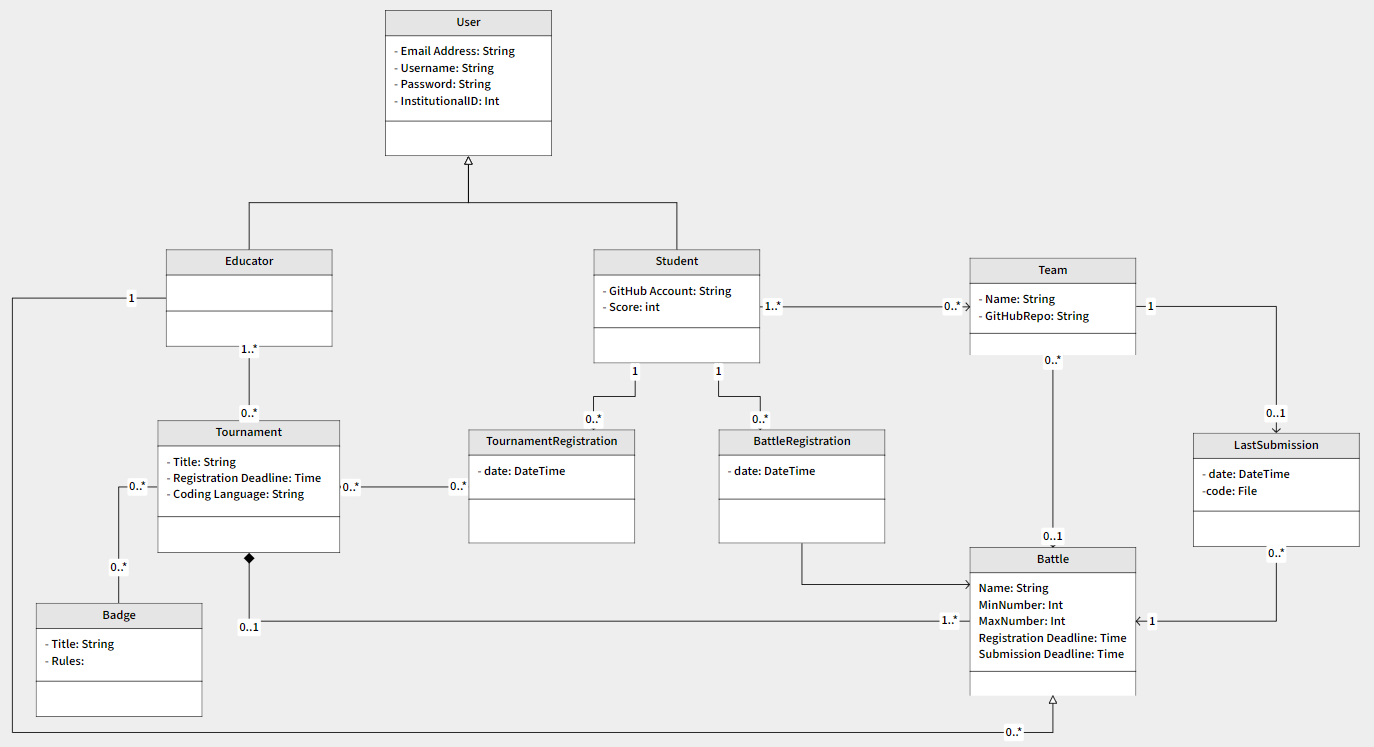
\includegraphics[width=1\linewidth]{Images/Diagrams/UML.png}
    \caption{UML}
    \label{fig:enter-label}
\end{figure}

\subsection{Product functions}

\begin{itemize}
    \item \textbf{Sign Up}$\\$This functionality allows Users to sign up on the CKB platform in order to use it. Once on the registration page, the user is asked if he/she wants to register as a student or as an educator. In the case of a student, the form requires an email address, which could be personal or institutional, a password, a GitHub account and other generic credentials to identify him/her (name, surname, student ID). Otherwise, the form asks the educator for his/her institutional email address, a password and other credentials to identify him/her (name, surname, educator ID for that specific school). The credentials then get verified and, if correct, the platform sends a confirmation email to the provided email address in order con confirm the registration. Once that’s done, the user is redirected to the login page. 
    \item \textbf{Tournament creation}$\\$This functionality allows educators to create a tournament through the CKB platform. From the main panel, educators can click the top-right “New Tournament” button and they get presented the dedicated pop-up page. Here the educator can set all the main parameters of the tournament like the name, the designated programming language (from a scroll-down menu), the deadline using a calendar view-like menu and an option tournament image. They proceed to the invitation form, where they can choose other educators to grant access to by searching their email address from a search bar and then pressing the “+” button on the side. Furthermore, they can scroll down and, by clicking the “Add Badge” button on the right of the “badge list” (supposed initially empty), can create custom badges for the specific tournament through a pop-up menu. Once the badge is created, it is shown in the “badge list”, which is a table showing the badge icon, badge name, rules and variables. When the creation is finished, the educator can click on “Save Changes” button on the bottom-left corner of the pup-up page. If there are no errors, the tournament is successfully created and published and the students get notified. 
    \item \textbf{Battle Creation}$\\$This functionality allows educators to create a battle for a tournament. From his/her personal main panel, an educator sees a list of all the open tournaments to which he/she has access; by clicking on a specific tournament's "Options" button, the educator is redirected to the Tournament Dashboard page, where he/she is presented with plenty of information such as a battle list, a scoreboard and much more. The educator then clicks on the “New Battle” button and is shown the battle creation pop-up page. Here the educator is asked to insert the battle name and number of students as well as, through some upload forms, all the files, information and test cases; CKB also asks for the two deadlines, inserted with the help of two calendar-view like menus, and for the quality aspects to keep track of during the evaluation of the projects proposed by the teams. Lastly, the educator clicks the "Save Changes" button in the bottom-left of the page and, if there are no errors, the educator is redirected to the Tournament Dashboard and a notification is sent to the students enrolled in that tournament, informing them of the newly created battle. 
    \pagebreak
    \item \textbf{Evaluation}$\\$This functionality is one of the most important in the CKB platform. Every time that a new push is detected, CKB pulls the latest version of the project from the GitHub repository and submits it to the uploaded test cases, which are run one by one by the automated scripts. To evaluate the project, which must receive a score between 0 and 100, CKB mostly uses automated evaluation criteria (which are mandatory): first of all, it measures how many test cases are passed successfully by the project, then it proceeds to measure how much time has passed between the registration deadline (same for all teams) and the last commit date. After that, based on the parameters selected by the educator when creating the battle, CKB must assert the quality level of the project's sources by making use of the static analysis tools integrated in the system; lastly, if selected, during the consolidation stage, an educator can modify the project's score on his/her own through the Evaluation Page. Once that is done, the CKB platform updates the final score for the team and the personal tournament score of each student accordingly. 
   \item \textbf{Badge Awarding}$\\$This functionality of the CKB platform grants a gamification aspect, useful to increase the feeling of achievement for the students participating in a tournament. The platform keeps track of various variables, defined by educators, throughout the whole tournament; these variables are used by the CKB platform to perform checks and verify if the rules, needed to achieve a certain badge, are satisfied. In case of all rules satisfied, the platform awards the badge to the corresponding student(s) by adding it to his/her/their personal page and by showing it on his/her/their public page. Students also get notified when they are awarded with a badge. 
   \item \textbf{Notification}$\\$This functionality is helpful for all Users, since it can provide various kind of information in a short time frame to a large number of receivers. Firstly, notifications are sent to users when they sign up to the platform, since they need to verify the profile through the link received by the email. Also educators when they get granted access to a tournament; students are also notified when a tournament is created and, if they subscribe to a tournament, get notified for every upcoming battle created in that tournament. Some students might get a notification if they are invited by their friends to join their team. CKB sends all subscribed students a notification when the GitHub repository is created and also, every time that a team pushes a new commit for a battle, notifies the students composing that team if their score has been improved. Something similar happens after the consolidation stage, only if the score of the team has been changed by an educator. At the end of each battle, the platform notifies subscribed students with their new tournament score and, lastly, at the end of the tournament, the students are notified as well. Students can, occasionally, get notifications if they are awarded with a badge. 
\end{itemize}

 \pagebreak
\subsection{User characteristics}
\begin{itemize}
    \item \textbf{Student}$\\$A student is a person who is enrolled in a school, has a device to connect to the internet and, more specifically, to the CKB platform. He/She uses the platform to join tournaments and battles, to form teams (according to the rules set by the educators) and, eventually, to see his/her score at the end of each battle. He/She also has the ability to invite his/her friends to join the same team to work together. 
    \item \textbf{Educator}$\\$ An educator is an adult who works in a school as a teacher and, thus, has some students enrolled on his courses. He/She has a device able to connect to internet and to the CKB platform so that he/she can create tournaments and/or battles, with all the required rules. He/She is also able to grant access to other educators to the tournament’s rules, so that they can help set it up and manage it. An educator can also inspect each team’s project, during the consolidation stage, to evaluate the project thoroughly in all its aspects. Moreover, an educator can create custom badges to assign to certain students who reach set achievements. 
    \item \textbf{User}$\\$A user can be either a student or an educator. He/She is able to register and to login onto the CKB platform in order to access its functions. If he/she is a “student”, the user is notified when the tournament is created and when its score is updated; if he/she is an “educator”, the user receives the notifications whenever the consolidation stage begins and manual evaluation is needed, as well as when the deadlines are reached. 
\end{itemize}

\subsection{Assumptions, dependencies and constraints}
The following assumptions are properties and/or conditions that the CKB platform takes for granted and that are necessary to reach the goals set. 

$\\$\textbf{[D1]}: Users must have a device able to connect to the internet. 
$\\$\textbf{[D2]}: Users give consent to the platform to receive notifications. 
$\\$\textbf{[D3]}: Students must have GitHub accounts. 
$\\$\textbf{[D4]}: Students must be enrolled in a school. 
$\\$\textbf{[D5]}: Students must provide correct and non fraudulent information during the registration and the login phase. 
$\\$\textbf{[D6]}: Students must grant access to their and only their GitHub account.
$\\$\textbf{[D7]}: Student must correctly fork the GitHub repository.

\clearpage

\section{Specific requirements}

\subsection{External interface Requirements}
\subsubsection{User Interfaces}

\begin{flushleft}
The following illustration depicts the platform's initial web page, which offers users the choice to either log in or sign up. [Fig.2]    
\end{flushleft}
\begin{figure}[htbp]
    \centering
    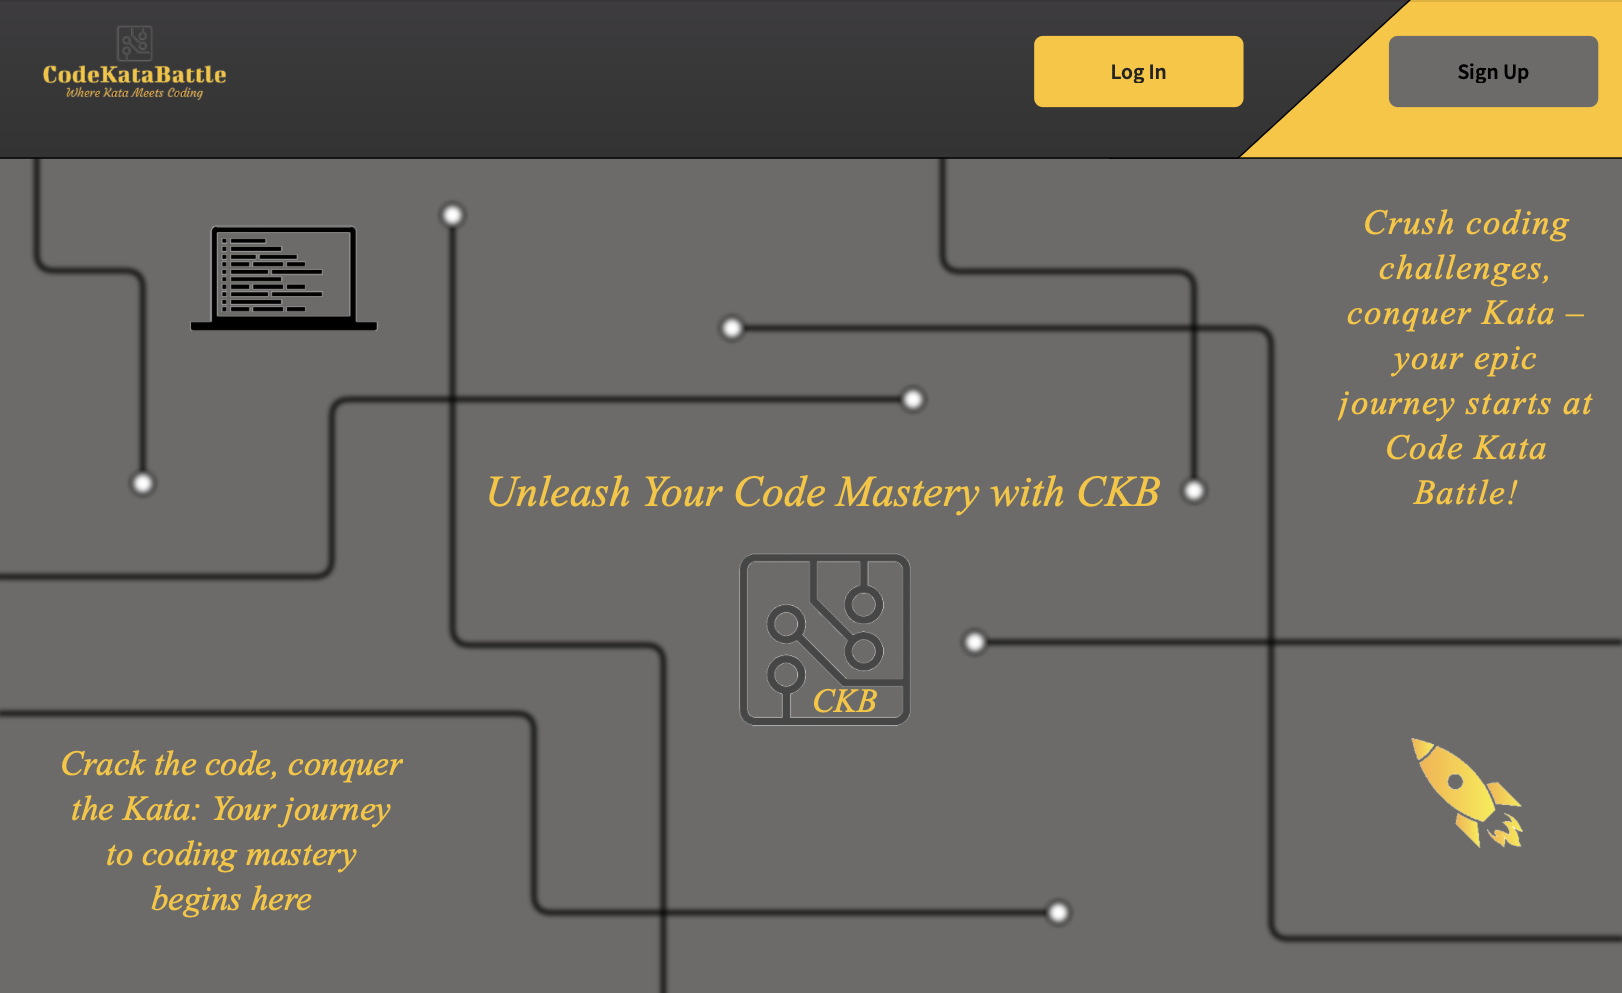
\includegraphics[width=1\linewidth]{Images/Interfaces/LandingPage.png}
    \caption{Landing page}
    \label{fig:enter-label}
\end{figure}

\clearpage

\begin{flushleft}
If the user opts to create an account, they will be prompted to input various details, including their username, email address, password, institutional id and an indication of their role as either an educator or a student. [Fig.3]    
\end{flushleft} 
\begin{figure}[htbp]
    \centering
    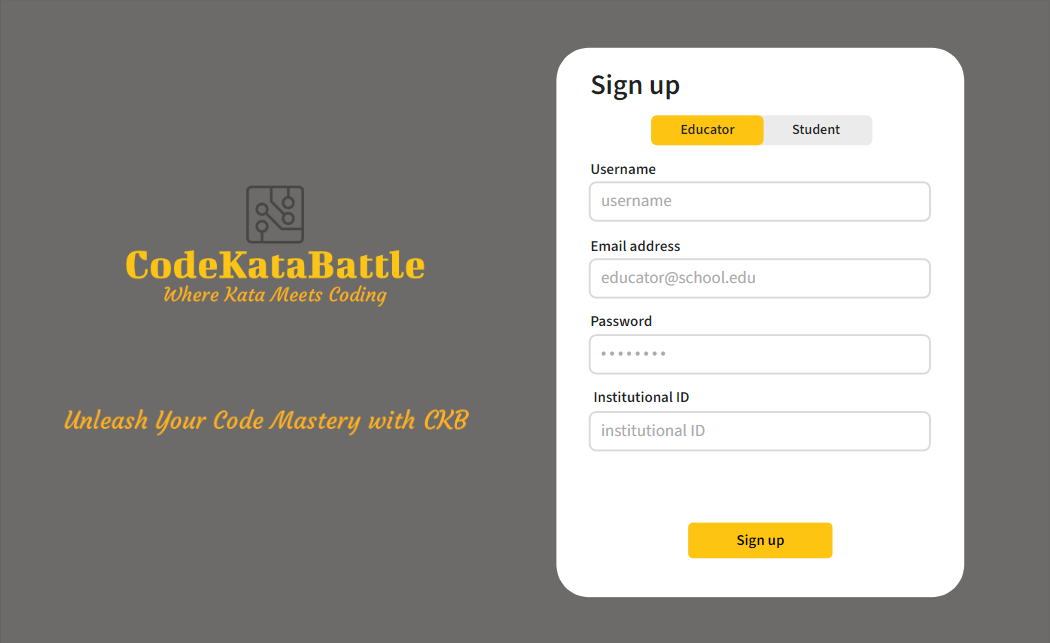
\includegraphics[width=1\linewidth]{Images/Interfaces/Educator Interfaces/EducatorSignUp.png}
    \caption{Sign up page - Educator}
    \label{fig:enter-label}
\end{figure}

\pagebreak

\begin{flushleft}
In the case of a student, there is an additional requirement to furnish information about their GitHub account. [Fig.4] 
\end{flushleft}
\begin{figure}[htbp]
    \centering
    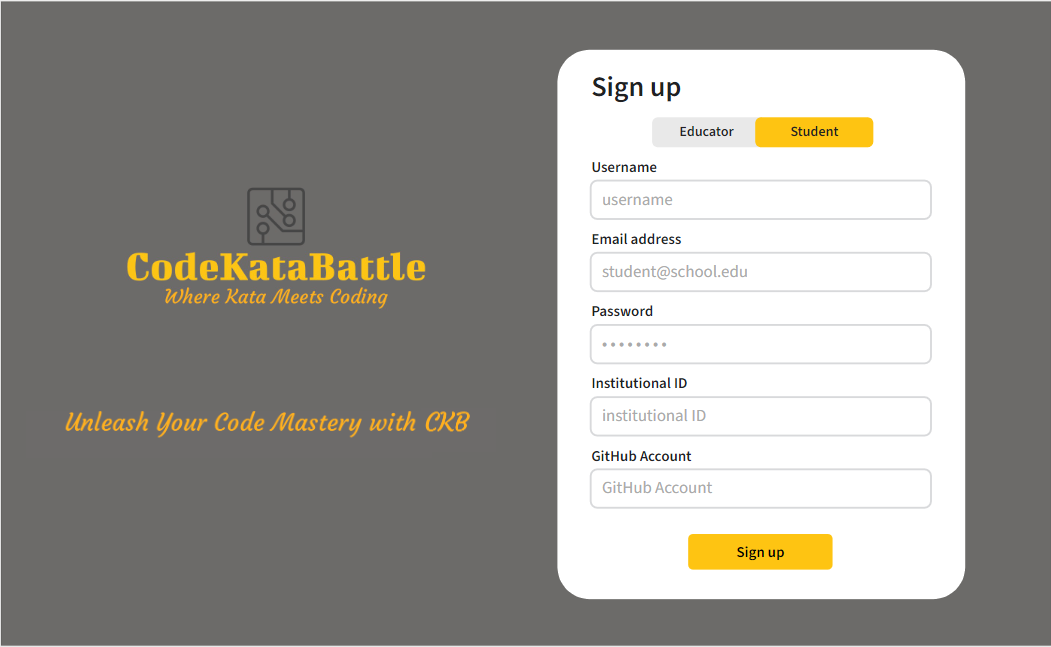
\includegraphics[width=1\linewidth]{Images/Interfaces/Student Interfaces/StudentSignUp.png}
    \caption{Sign up page - Student}
    \label{fig:enter-label}
\end{figure}

\pagebreak

\begin{flushleft}
For users who already have an account, accessing the platform is as simple as providing their username and password. Additionally, there's an option to enable the "Remember me" feature, which eliminates the need for repeated logins in the future. [Fig.5]    
\end{flushleft}

\begin{figure}[htbp]
    \centering
    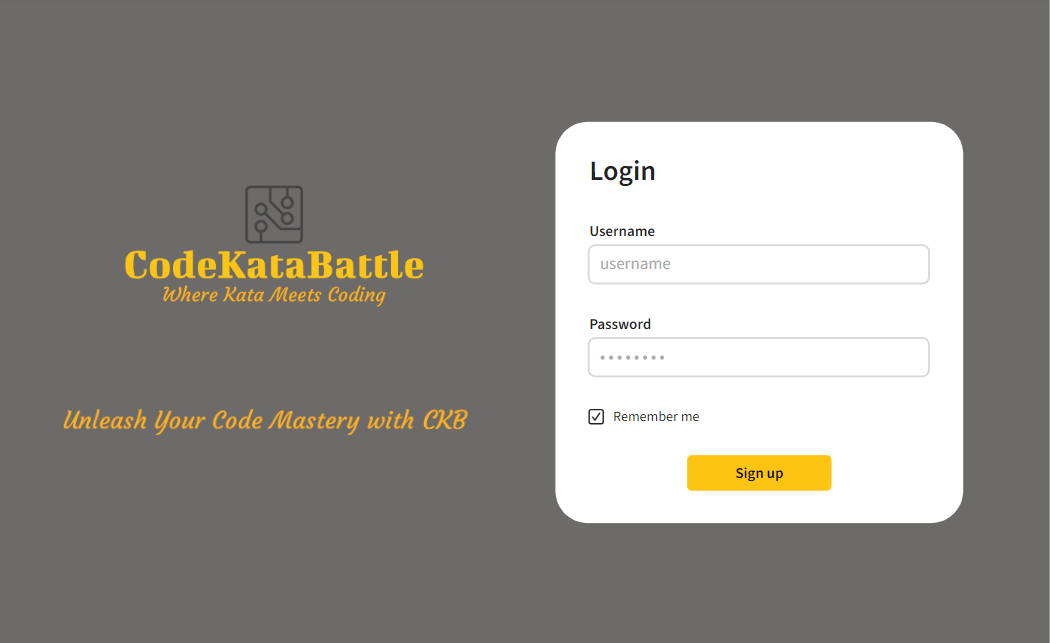
\includegraphics[width=1\linewidth]{Images/Interfaces/Login.png}
    \caption{Login page}
    \label{fig:enter-label}
\end{figure}

\pagebreak

\subsubsection{Educator Interfaces}
\begin{flushleft}
The educator dashboard, depicted in the illustration below [Fig. 6], provides a comprehensive view. Here, educators can effortlessly access useful information such as the total number of enrolled students, badges awarded, and a complete list of administered tournaments and their main parameters. Notably, educators also have the capability to seamlessly create new tournaments, see a specific tournament's page or close an open tournament, enhancing their control and management capabilities.    
\end{flushleft}

\begin{figure}[htbp]
    \centering
    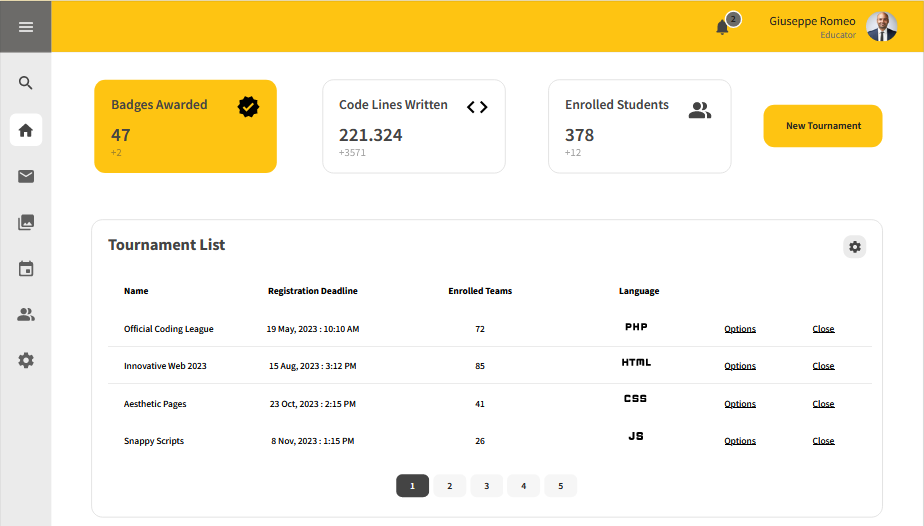
\includegraphics[width=1\linewidth]{Images/Interfaces/Educator Interfaces/EducatorDashboard.PNG}
    \caption{Educator Dashboard}
    \label{fig:enter-label}
\end{figure}

\pagebreak

\begin{flushleft}
The illustrations below [Fig.7] demonstrate the user-friendly process through which educators can effortlessly initiate a new tournament. Within this intuitive interface, educators have the flexibility to select the tournament's name, coding language requirements for students, registration deadline, tournament picture, badge list, and even invite specific educators to access and contribute to the tournament formation.    
\end{flushleft}

\begin{figure}[htbp]
    \centering
    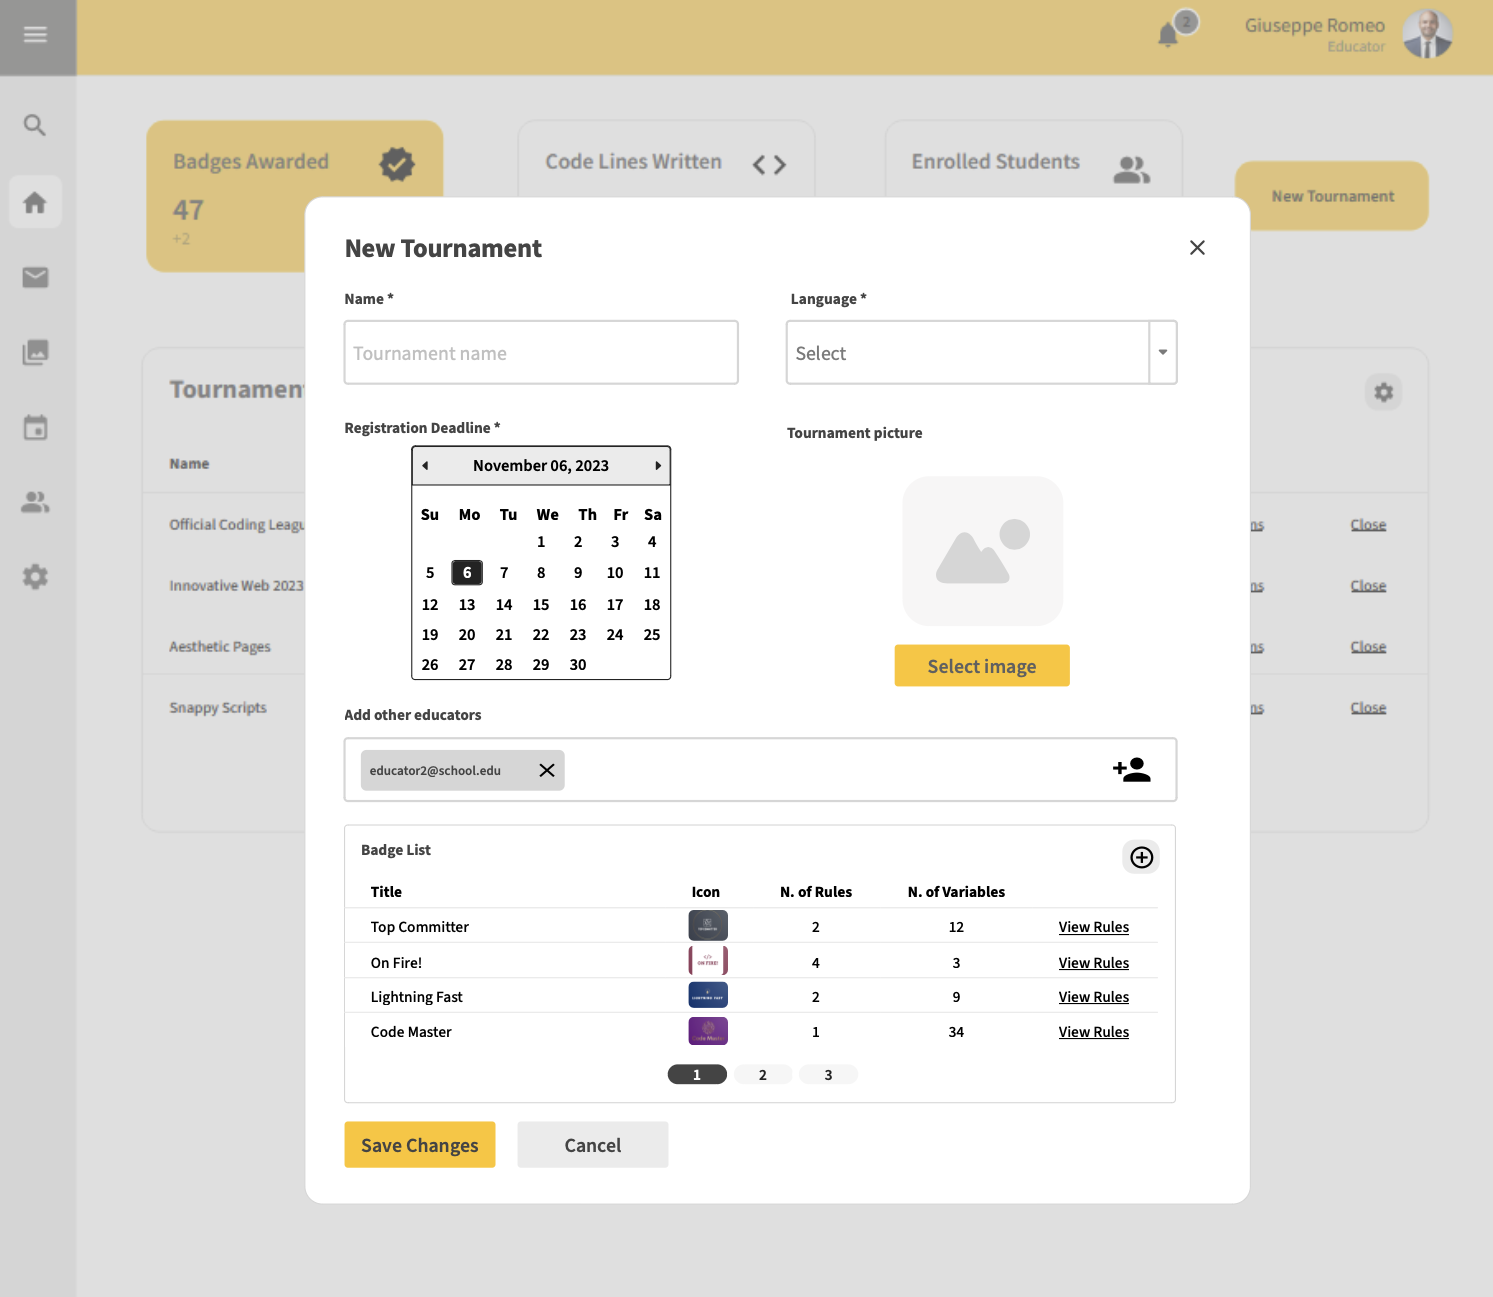
\includegraphics[width=1\linewidth]{Images/Interfaces/Educator Interfaces/CreateTournament.png}
    \caption{Tournament Creation}
    \label{fig:enter-label}
\end{figure}

\pagebreak

\begin{flushleft}
In the domain of badge creation, educators have the ability showcased in [Fig. 8]. Here, they can craft badges to be awarded to the students who accomplish them. With a few clicks, educators choose the badge's icon and name, while also defining the specific criteria students must fulfill to earn the badge. It's a seamless process that adds a touch of recognition to student achievements.    
\end{flushleft}

\begin{figure}[htbp]
    \centering
    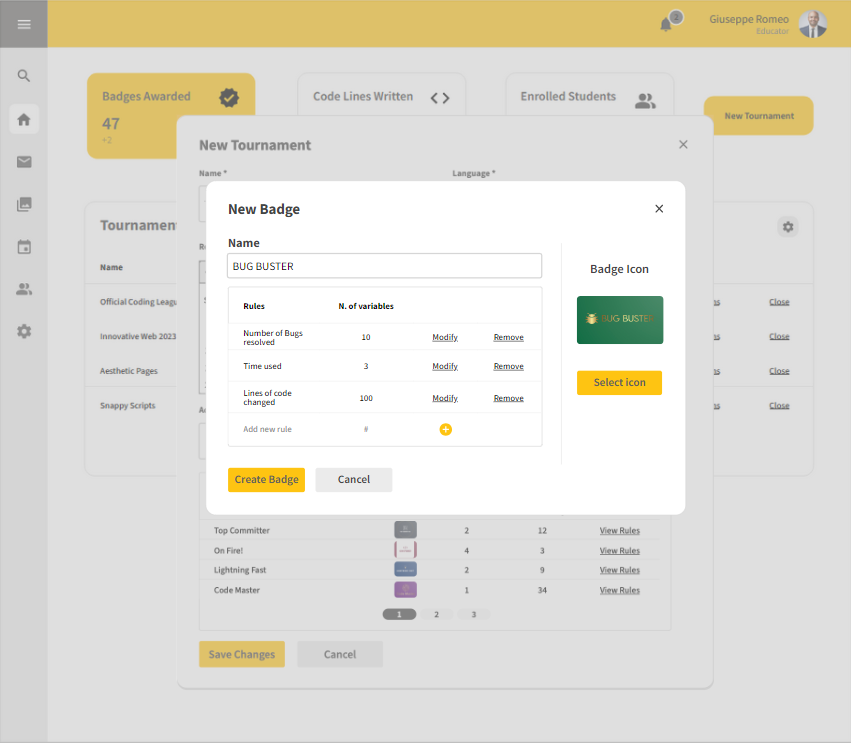
\includegraphics[width=1\linewidth]{Images/Interfaces/Educator Interfaces/CreateBadge.png}
    \caption{Badge Creation}
    \label{fig:enter-label}
\end{figure}

\pagebreak

\begin{flushleft}
The illustrations below [Fig.9] shows the tournament dashboard that the educator who created that tournament and the colleagues who have the permission can access. It provides tons of information like the battle list with respective parameters and options, the scoreboard and much more.   
\end{flushleft}

\begin{figure}[htbp]
    \centering
    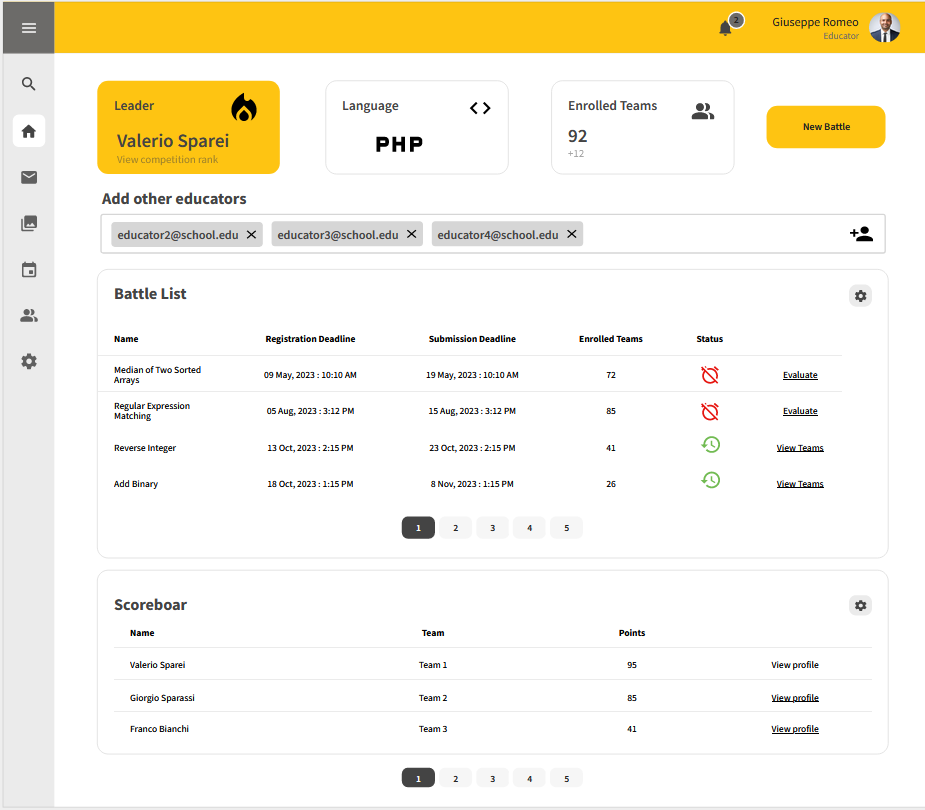
\includegraphics[width=1\linewidth]{Images/Interfaces/Educator Interfaces/EducatorTournDash.PNG}
    \caption{Educator Tournament Dashboard}
    \label{fig:enter-label}
\end{figure}

\pagebreak

\begin{flushleft}
Educators take charge of crafting individual battles within the tournament, as depicted in the illustrative image below [Fig. 10]. During battle creation, they wield the power to determine the battle's name, set the minimum and maximum number of students per group, specify registration and submission deadlines, and furnish a comprehensive battle description. At the bottom of the interface, educators can fine-tune the evaluation process by selecting specific aspects (such as Security, Reliability, Maintainability) to consider, and they have the option to manually assess scores post-battle. To streamline the evaluation, educators can effortlessly upload test cases and the script, automating the assessment based on the provided test cases.   
\end{flushleft}

\begin{figure}[htbp]
    \centering
    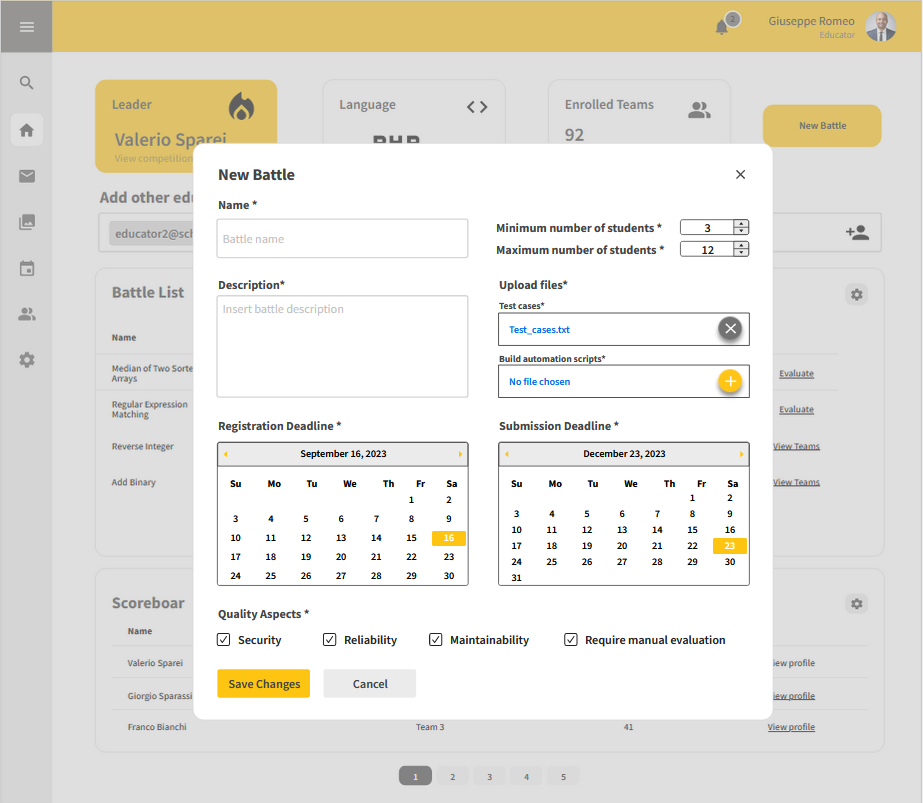
\includegraphics[width=1\linewidth]{Images/Interfaces/Educator Interfaces/BattleCreation.PNG}
    \caption{Battle Creation}
    \label{fig:enter-label}
\end{figure}

\pagebreak

\begin{flushleft}
Finally, educators can access the view presented in [Fig. 11], showcasing individual battles undertaken by students. Within this page, they gain insights into group performance through informative charts, detailing Timeliness and the aspects considered during battle creation. The platform autonomously generates a final score, and if the manual scoring option was selected, educators can manually adjust the scores. For informed decision-making, a click of a button seamlessly directs them to the GitHub repository, allowing a thorough review of the code written by the student teams.    
\end{flushleft}

\begin{figure}[htbp]
    \centering
    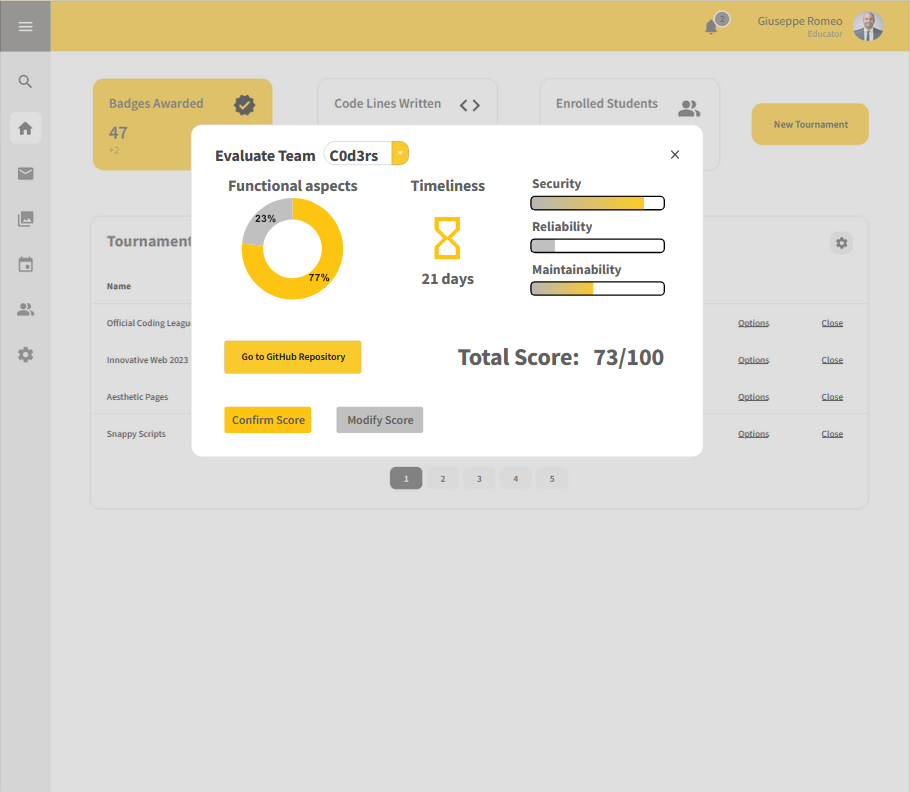
\includegraphics[width=1\linewidth]{Images/Interfaces/Educator Interfaces/EvaluationPage.png}
    \caption{Evaluation Page}
    \label{fig:enter-label}
\end{figure}

\pagebreak

\subsubsection{Student Interfaces}
\begin{flushleft}
The student dashboard, as depicted in the visual aid [Fig. 12], provides a comprehensive snapshot of the student's journey. Through intuitive pie charts, it showcases the tournaments and battles the student is currently enrolled in, along with those successfully completed. Additionally, the dashboard highlights the number of badges achieved and the quantity of code lines written by the student. For seamless continuity, the student can easily navigate to their GitHub profile and navigate the tournaments directly from the displayed list.    
\end{flushleft}

\begin{figure}[htbp]
    \centering
    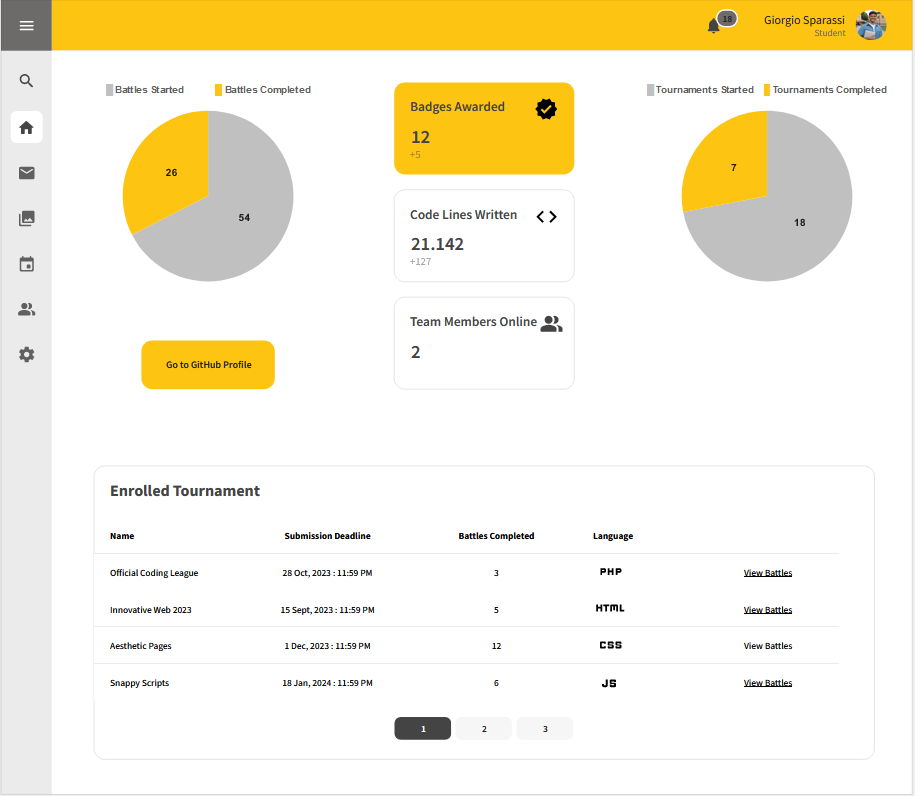
\includegraphics[width=1\linewidth]{Images/Interfaces/Student Interfaces/StudentDash.PNG}
    \caption{Student Dashboard}
    \label{fig:enter-label}
\end{figure}

\pagebreak

\begin{flushleft}
Given that students require an invitation from the educator to enroll in the tournaments, their participation is limited to joining individual battles. As depicted in [Fig. 13], students enrolled in a tournament gain access to a comprehensive list of battles within the tournament, complete with registration and submission deadlines, along with a scoreboard indicating the top performing students for that tournament.   
\end{flushleft}

\begin{figure}[htbp]
    \centering
    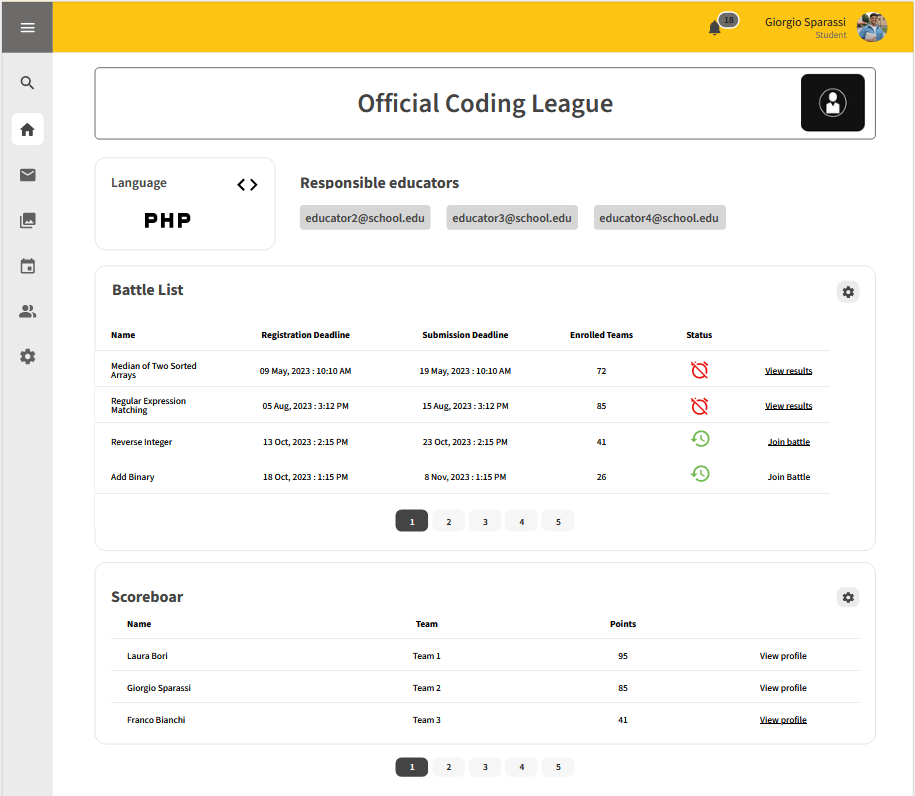
\includegraphics[width=1\linewidth]{Images/Interfaces/Student Interfaces/TournamentDashboard.PNG}
    \caption{Tournament Dashboard}
    \label{fig:enter-label}
\end{figure}

\pagebreak

\begin{flushleft}
As shown in [Fig. 14], students enrolled in a tournament can join an open battle, either alone of by inviting friends and, thus, creating a new team for that battle.  
\end{flushleft}

\begin{figure}[htbp]
    \centering
    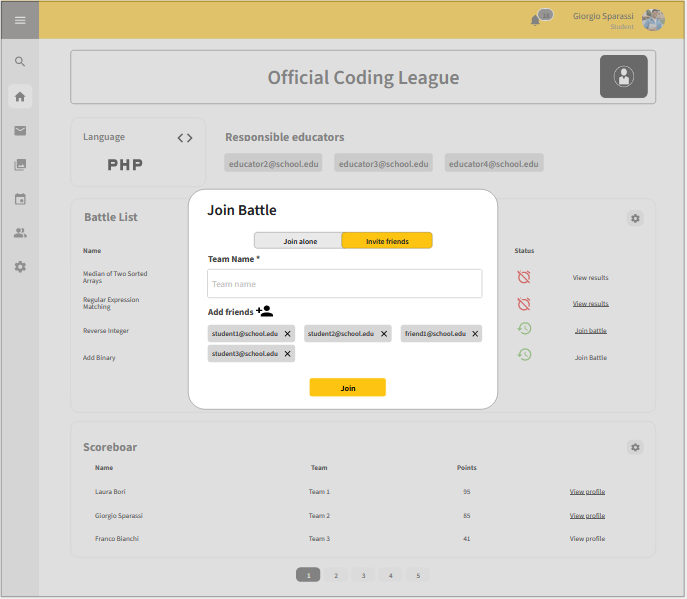
\includegraphics[width=1\linewidth]{Images/Interfaces/Student Interfaces/JoinBattleStud.PNG}
    \caption{Student joining a battle}
    \label{fig:enter-label}
\end{figure}

\pagebreak

\begin{flushleft}The visual representation in [Fig. 15] illustrates the students' engagement in battles. It presents a detailed description of the battle, including its constraints. To aid students, there are examples and starter lines of code. The required programming language is highlighted, and informative charts display the number of passed and failed test cases, as well as the student's coding activity, including lines written and deleted. With a simple button press, students can seamlessly transition to their GitHub repository to commence coding and invite other students to join their group. At the bottom, students can seamlessly navigate through the battles within the tournament.
\end{flushleft}

\begin{figure}[htbp]
    \centering
    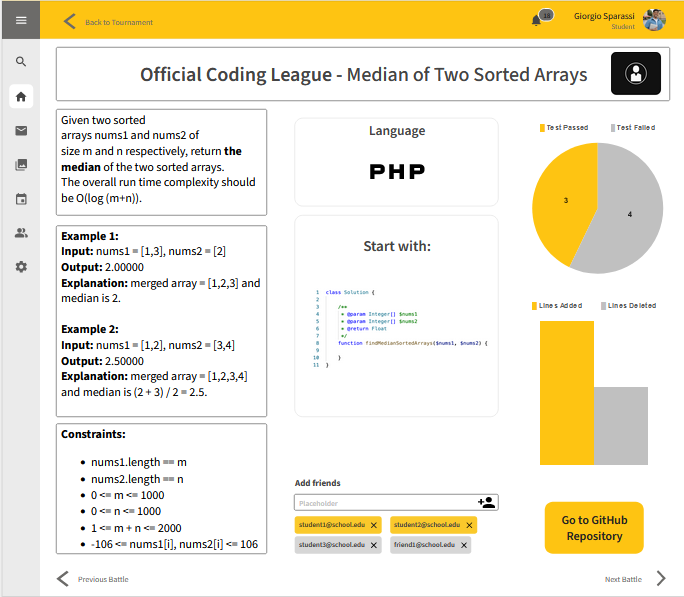
\includegraphics[width=1\linewidth]{Images/Interfaces/Student Interfaces/OngoingBattle.PNG}
    \caption{Battle Description}
    \label{fig:enter-label}
\end{figure}

\pagebreak

\subsubsection{Hardware Interfaces}
The platform exclusively operates online, serving as a web-based platform where users engage through their personal computers or a mobile device. It does not offer any hardware interface. 

\subsubsection{Software Interfaces}
As a software interface, the system instructs students to fork the GitHub repository of the code kata. It also facilitates the configuration of an automated workflow utilizing GitHub Actions. This workflow is designed to interact with the CKB platform through appropriate API calls whenever students make new commits to the main branch of their repository.  
This interface ensures seamless coordination between students, GitHub Actions, and the CKB platform, streamlining the process of code analysis. Through the static analysis tools the platform automatically evaluates the team score following the criteria chosen by the evaluator.
 
\subsubsection{Communication Interfaces}
Regarding communication interfaces, the system establishes a directional connection between GitHub Actions and the CKB platform. This communication enables GitHub Actions to effectively transmit the necessary data and notifications to the CKB platform whenever new commits occur from students. Communication between these components is crucial for ensuring a smooth flow of information and effective management of scoring and analysis within the system. 

\clearpage

\subsection{Functional Requirements}

\subsubsection{Use Case}

\begin{table}[htbp]
\begin{tabular}{|l|p{12cm}|}
    \hline
    \multicolumn{2}{|l|}{\textbf{[UC1] User Registration}}\\
    \hline
    Actors & User\\
    \hline
    Entry condition & User has navigated to the landing page.\\
    \hline
    Input & The system asks for User username, User email, User password, User institutional ID.
    \\
    \hline
    Event flow & The user clicks on the top-right "Sign Up" button. The platform displays the "Sign Up" page and the user has to choose whether to sign up as a "Student" or as an "Educator". After that, he/she proceeds to insert all the needed data in the respective text boxes, displayed by the system. Once the user has inserted all the mandatory data, he/she clicks on the "Sign up" button on the bottom of the page. The platform displays the acceptance of registration and invites the user to confirm the registration by clicking the link provided in the email, sent by the platform.\\
    \hline
    Exit condition & User inserted data are valid and correct. User registration has been successful.\\
    \hline
    Output & The user's data are stored in the system's database and the user receives the confirmation email.
    \\
    \hline
    Exceptions & \begin{itemize}
        \item If the username input by the user upon registration is already taken by someone else, the platform aborts the registration, prompts an error to the user and asks him/her to insert a different username.
        \item If the inserted institutional ID is invalid, has wrong length or belongs to a different type of user (i.e. a "student" tries to register using an educator's ID), the platform aborts the registration, prompts an error to the user and asks him/her to insert a valid institutional ID.
        \item If the inserted email address is invalid or has already been used, the platform aborts the registration, prompts an error to the user and asks him/her to insert a valid email address.
    \end{itemize}\\
    \lasthline
\end{tabular}
\end{table}
\clearpage

\begin{figure}[htbp]
    \centering
    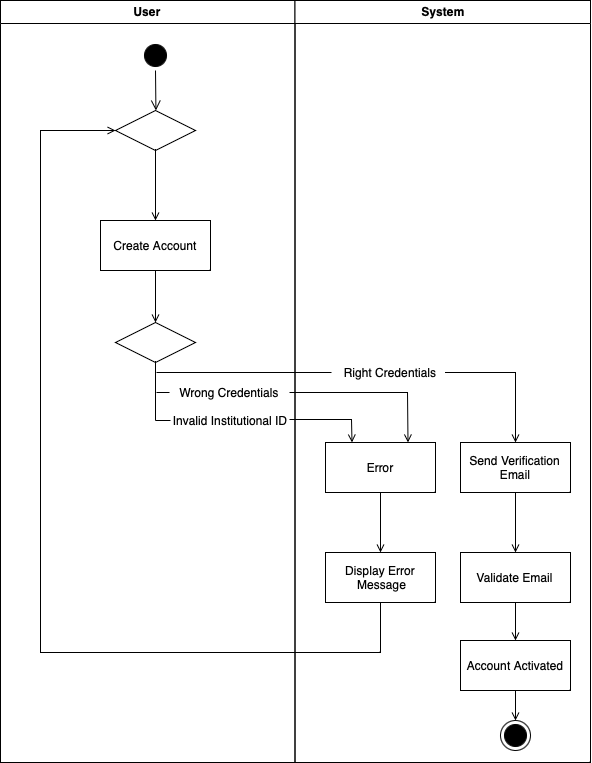
\includegraphics[width=1\linewidth]{Images/Diagrams/UserRegistration.png}
    \caption{Diagram for [UC1]}
    \label{fig:enter-label}
\end{figure}

\clearpage

\begin{table}[htbp]
\begin{tabular}{|l|p{12cm}|}
    \hline
    \multicolumn{2}{|l|}{\textbf{[UC2] User Login}}\\
    \hline
    Actors & User\\
    \hline
    Entry condition & User has navigated to the landing page\\
    \hline
    Input & \begin{itemize}
        \item Username
        \item Password
    \end{itemize}\\
    \hline
    Event flow & The User clicks on the top-right "Log in" button. The platform displays the "Log In" page and the user insert all the needed data in the respective text boxes, displayed by the system. Once the user has inserted all the mandatory data, he/she clicks on the "Log In" button on the bottom of the page.
    The system checks the correctness of the credentials inserted and redirect to the home page.\\
    \hline
    Exit condition & User is logged in\\
    \hline
    Exception & \begin{itemize}
        \item If the username inserted is not registered in the platform's database, the platform prompts an error to the user and asks him/her to insert a registered username.
        \item If the password inserted doesn't match with the one associated with the inserted username in the platform's database, the platform prompts an error to the user and asks him/her to insert the correct password.
    \end{itemize}\\
    \lasthline
\end{tabular}
\end{table}

\begin{figure}[htbp]
    \centering
    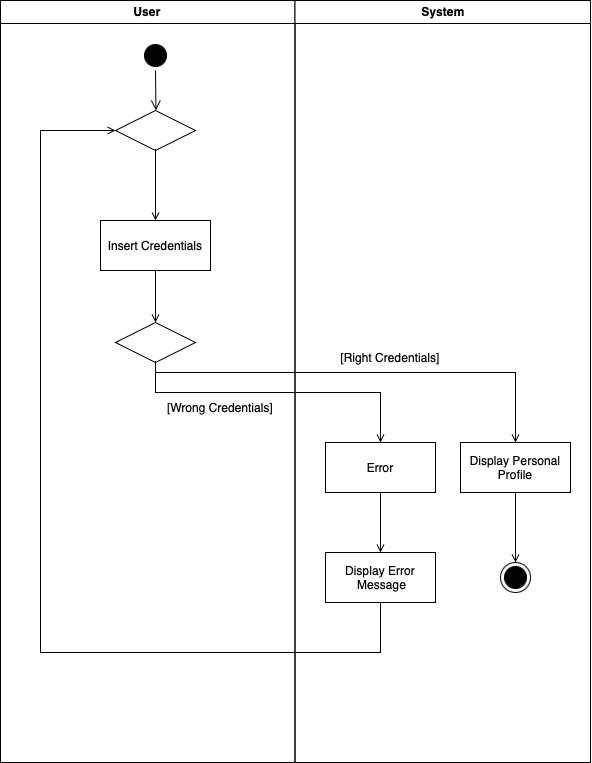
\includegraphics[width=1\linewidth]{Images/Diagrams/LogIn.png}
    \caption{Diagram for [UC2]}
    \label{fig:enter-label}
\end{figure}

\begin{table}[htbp]
\begin{tabular}{|l|p{12cm}|}
    \hline
    \multicolumn{2}{|l|}{\textbf{[UC3] Educator creates a tournament}}\\
    \hline
    Actors & Educator\\
    \hline
    Entry condition & Educator, who is already logged in, has navigated to the "Educator dashboard" page.\\
    \hline
    Input & Optionally, other educators' email addresses\\
    \hline
    Event flow &  The Educator clicks on the "New Tournament" button on the top-right side of the page. The "New Tournament" pop-up page is displayed by the platform. The educator inserts the tournament name in the designed text-box and chooses the programming language of the tournament from the drop-down menu; also, from the calendar-view menu, he/she selects the registration deadline. The educator can as well upload an image and make it the tournament picture. Optionally, the educator can grant permission to other educators by typing their email addresses inside the text-box and clicking the button on the right. If the address is incorrect, or the educator changes his/her mind, it can be deleted by clicking the "x" button. Moreover, the educator can insert one or more badges by clicking the "+" button inside the "Badge List". From there, he/she can click on the "Choose Existing" button to add an existing badge or create a new one from scratch by clicking "New Badge". The educator clicks on the "Save Changes" button on the bottom-left of the pop-up page. \\
    \hline
    Exit condition & All mandatory data are inserted. Inserted data are correct and valid.\\
    \hline
    Output & \begin{itemize}
        \item The tournament is created
        \item The tournament invitation link is sent by email to all the students.
        \item Optionally, permission-granting emails are sent to the selected educators.
    \end{itemize}\\
    \hline
    Exception & \begin{itemize}
        \item If the name inserted has already been assigned to another tournament, the platform prompts an error to the educator and asks him/her to insert a valid name.
        \item If the registration deadline set by the educator is prior to the current date detected by the platform, the platform prompts an error to the educator and asks him/her to insert a valid deadline.
    \end{itemize}\\
    \lasthline
\end{tabular}
\end{table}

\begin{figure}[htbp]
    \centering
    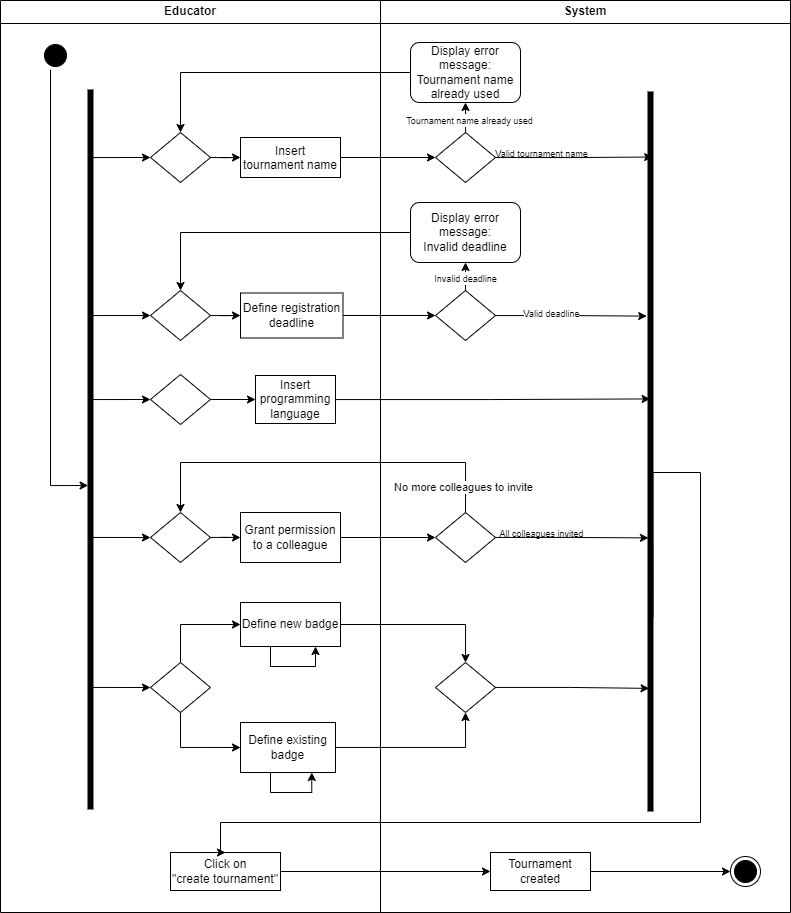
\includegraphics[width=1\linewidth]{Images/Diagrams/EducatorCreatesTournament.png}
    \caption{Diagram for [UC3]}
    \label{fig:enter-label}
\end{figure}

\pagebreak

\begin{table}[htbp]
\begin{tabular}{|l|p{12cm}|}
    \hline
    \multicolumn{2}{|l|}{\textbf{[UC4] Educator creates a badge}}\\
    \hline
    Actors & Educator\\
    \hline
    Entry condition & Educator, who is already logged in, is creating a tournament\\
    \hline
    Input & \begin{itemize}
        \item Badge Name
        \item Rules
        \item Image
    \end{itemize}\\
    \hline
    Event flow & The Educator clicks on the button "+" and clicks on the "New Badge" button. He/she inserts the name of the new badge and defines the rules and the relative number of variables by clicking the "+" button. The educator can either select an existing rule or create a new one. If the educator wants to change a rule, he/she can click on "Modify" and change the number of the variables. A rule can be removed by clicking on the "Remove" button. Finally, the educator can add an icon to represent the badge. When all the information are inserted, the educator clicks on "Create Badge".\\
    \hline
    Exit condition & The system displays the previous page of creation of the tournament with the new badge added.\\
    \hline
    Output & The system stores the new badge.\\
    \hline
    Exception & If the name inserted already belongs to another badge, the system highlights the textbox of the name and asks to insert a different one.\\
    \lasthline
\end{tabular}
\end{table}

\begin{figure}[htbp]
    \centering
    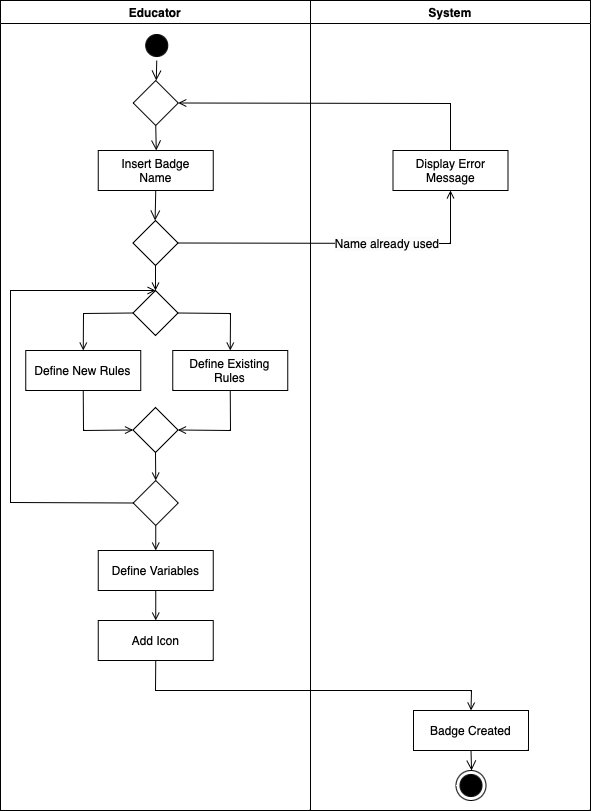
\includegraphics[width=1\linewidth]{Images/Diagrams/CreateBadges.png}
    \caption{Diagram for [UC4]}
    \label{fig:enter-label}
\end{figure}

\pagebreak

\begin{table}[htbp]
\begin{tabular}{|l|p{12cm}|}
    \hline
    \multicolumn{2}{|l|}{\textbf{[UC5] Educator grants permission to a colleague}}\\
    \hline
    Actors & Educator\\
    \hline
    Entry condition & Educator, who is already logged in, has navigated to the "Educator dashboard" page.\\
    \hline
    Input & Other educators' email addresses\\
    \hline
    Event flow & The educator who created the tournament clicks on the "Options" button, placed in the "Tournament List". From the now opened "Tournament Dashboard", the educator inserts the email addresses in the shown text-box one by one and clicks on the button on the right of the text-box. Also here, If the address is incorrect, or the educator changes his/her mind, it can be deleted by clicking the "x" button.\\
    \hline
    Exit condition & The educator clicks on the "Save Changes" button.\\
    \hline
    Output & Permission-granting emails are sent to the selected educators.\\
    \hline
    Exception & If the email address inserted by the educator is incorrect, or is not associated to any educator, the platform display an error message and asks the educator to insert a valid address.\\
    \lasthline
\end{tabular}
\end{table}

\begin{figure}[htbp]
    \centering
    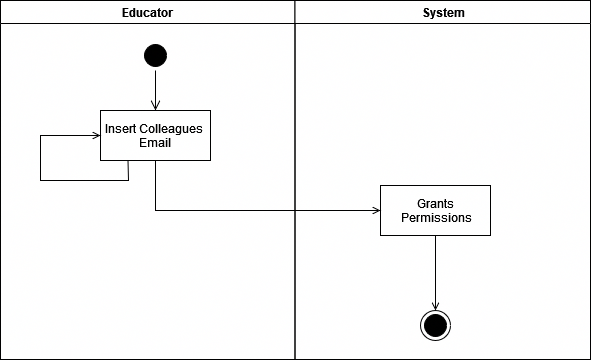
\includegraphics[width=1\linewidth]{Images/Diagrams/GrantPermission.png}
    \caption{Diagram for [UC5]}
    \label{fig:enter-label}
\end{figure}

\clearpage

\begin{table}[htbp]
\begin{tabular}{|l|p{12cm}|}
    \hline
    \multicolumn{2}{|l|}{\textbf{[UC6] Student enrolls in a tournament}}\\
    \hline
    Actors & Student\\
    \hline
    Entry condition & The Educator created a tournament\\
    \hline
    Event flow & The student clicks on the link provided in the email sent by the platform. He/she clicks on the link and, if there are no connection error and he/she does so before the registration deadline, he/she gets enrolled in the tournament.\\
    \hline
    Exit condition & Student is successfully enrolled in the tournament.\\
    \hline
    Output & Student receives a notification whenever a new battle in the tournament is created.\\
    \hline
    Exception & If the registration deadline has been reached, the platform prompts an error message, denying the tournament registration.\\
    \lasthline
\end{tabular}
\end{table}

\begin{figure}
    \centering
    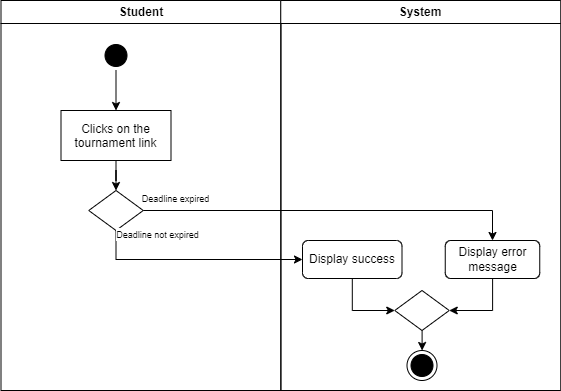
\includegraphics[width=1\linewidth]{Images//Diagrams/StudentsEnrollsTournament.png}
    \caption{Diagram for [UC6]}
    \label{fig:enter-label}
\end{figure}

\clearpage

\begin{table}[htbp]
\begin{tabular}{|l|p{12cm}|}
    \hline
    \multicolumn{2}{|l|}{\textbf{[UC7] Educator creates a battle}}\\
    \hline
    Actors & Educator\\
    \hline
    Entry condition & Educator, who is already logged in, has navigated to the "Educator dashboard" page.\\
    \hline
    Event flow & The educator clicks on the "Options" button, located in the "Tournament List". The platform displays the "Tournament Dashboard" page. The educator click on the top-right "New Battle" button. The "New Battle" pop-up page is shown. Firstly, the educator writes down the battle name in the designated field, then he/she chooses the minimum and maximum number of students allowed for each team. The educator proceed with writing the description of the battle and uploads the test cases and the automation scripts, by making use of the upload forms displayed. From the calendar-view menus he/she sets both the registration and submission deadlines and, lastly, selects from the checkboxes the quality aspects that the platform has to consider when evaluating a project, as well as the optional manual review.\\
    \hline
    Exit condition & All mandatory data are inserted. Inserted data are correct and valid.\\
    \hline
    Output & \begin{itemize}
        \item The battle is created
        \item The platform sends, to every student enrolled in the tournament for which the battle was created, a notification
    \end{itemize}\\
    \hline
    Exception & \begin{itemize}
        \item If the battle's name has already been taken, the platform prompts an error to the educator and asks him/her to insert a valid name.
        \item If the maximum number of students is inferior to the minimum number, or viceversa, the platform prompts an error to the educator and asks him/her to insert valid values.
        \item If the one or both the deadlines are set before the current date, detected by the platform, the platform prompts an error to the educator and asks him/her to insert a valid deadline.
        \item If the submission deadline is set prior to the registration deadline, the platform prompts an error to the educator and asks him/her to insert a valid deadline.
        \item If one or more mandatory files to upload are missing, the platform prompts an error to the educator and asks him/her to upload the missing files.
    \end{itemize}\\
    \lasthline
\end{tabular}
\end{table}

\begin{figure}
    \centering
    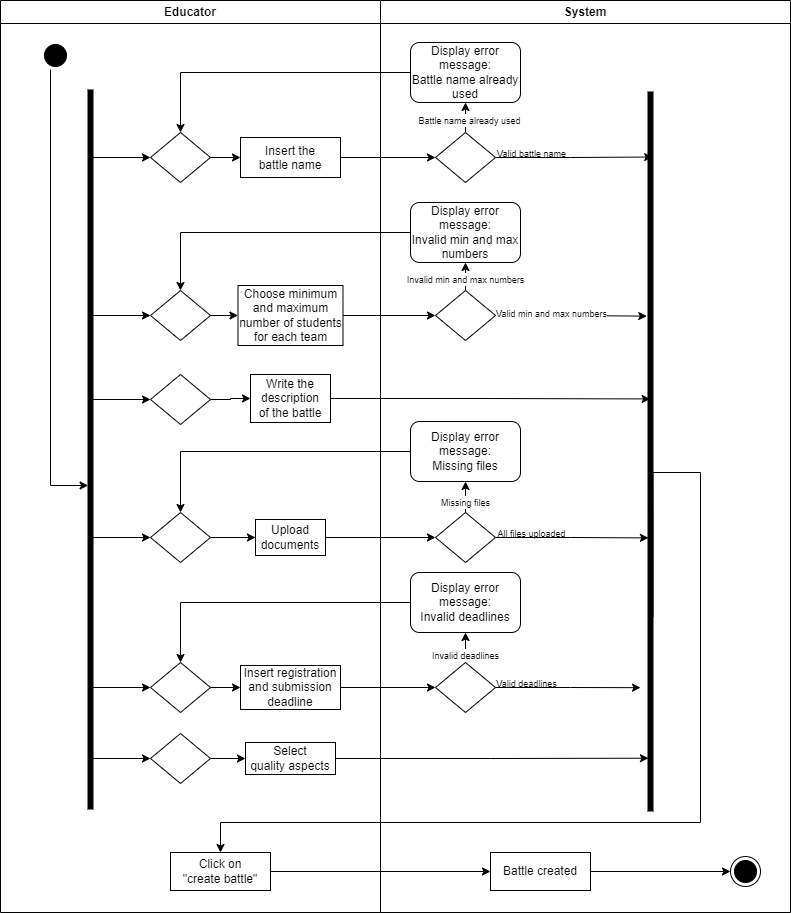
\includegraphics[width=1\linewidth]{Images//Diagrams/EducatorCreatesBattle.png}
    \caption{Diagram for [UC7]}
    \label{fig:enter-label}
\end{figure}

\pagebreak

\begin{table}[htbp]
\begin{tabular}{|l|p{12cm}|}
    \hline
    \multicolumn{2}{|l|}{\textbf{[UC8] Student enrolls to a battle}}\\
    \hline
    Actors & Student\\
    \hline
    Entry condition & Student, who is already logged in, has navigated to the "Tournament dashboard" page.\\
    \hline
    Event flow &  The student clicks on the "Join battle" button and decides whether if he/she wants to join alone the battle or if he/she wants to invite some friends. In both cases the student must insert a name for his/her team. Once submitted the name, if the student is alone, he/she doesn't have to insert other information. Otherwise the student can specify the email addresses of the friends he/she wants to invite. The invitations can be also removed by clicking the "x" symbol next to each email address. The friends who receive the invitation can join the battle as specified in [UC10]\\
    \hline
    Exit condition & The student clicks on the "Join" button\\
    \hline
    Output & The system stores the new team and the partecipants.\\
    \hline
    Exceptions &
    \begin{itemize}
        \item The student wants to join the battle with a number of teammates that is not allowed. In this case the system tells the user how many students for each team are allowed, and let the user change the invitations.
        \item The student insert a team name which already belongs to another team. In this case the system highlights the textbox of the name and asks to insert a different name.
    \end{itemize}\\
    \lasthline
\end{tabular}
\end{table}

\clearpage

\begin{figure}
    \centering
    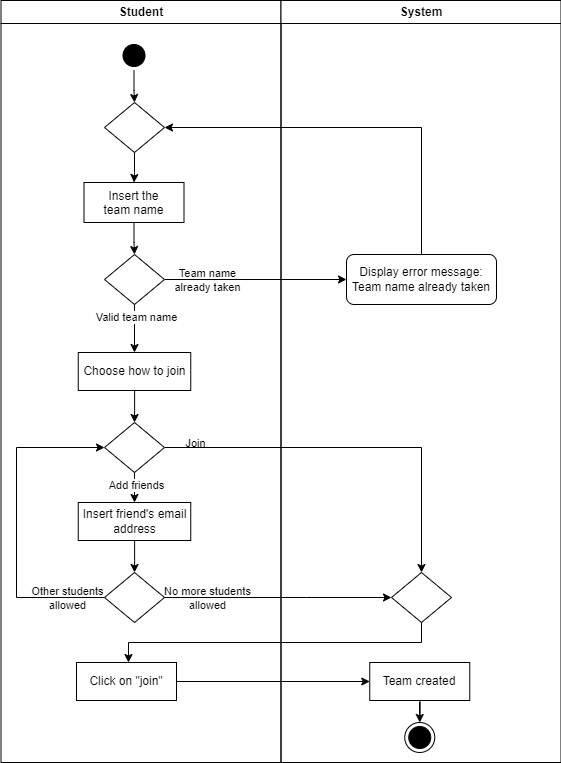
\includegraphics[width=1\linewidth]{Images//Diagrams/StudentEnrollsBattle.png}
    \caption{Diagram for [UC8]}
    \label{fig:enter-label}
\end{figure}

\clearpage

\begin{table}[htbp]
\begin{tabular}{|l|p{12cm}|}
    \hline
    \multicolumn{2}{|l|}{\textbf{[UC9] Student invites a friend to join his/her team}}\\
    \hline
    Actors & Student\\
    \hline
    Entry condition & Student, who is already logged in, has navigated to the "Tournament dashboard" page.\\
    \hline
    Event flow & The Student selects a battle from the battle list to see the details. He/she insert on the textbox at the bottom of the page the email address of the friend he/she wants to invite and clicks on the icon on the right. Yellow colored email addresses belong to the students who accepted the invitation and are effectively part of the team; the grey colored are the email addresses of the students who received the invitation but that didn't accepted yet.\\
    \hline
    Exit condition & The student clicks on the icon at the right of the textbox\\
    \hline
    Exception & The student inserts the email address of a friend who is already part of another team in the same battle. In this case the system highlights in red the textbox and inform the user that he/she can't invite the user he/she mentioned\\
    \lasthline
\end{tabular}
\end{table}

\clearpage

\begin{figure}
    \centering
    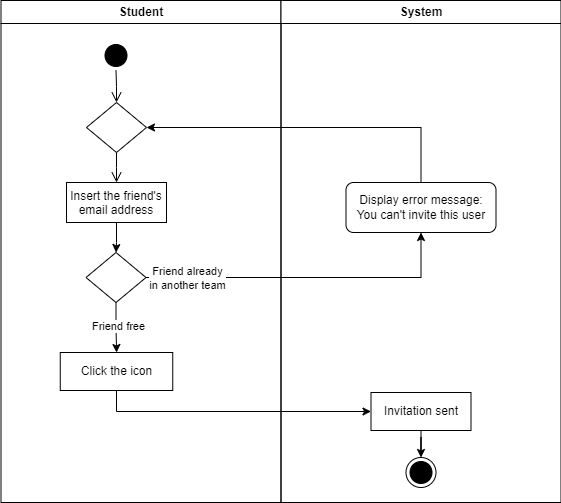
\includegraphics[width=1\linewidth]{Images//Diagrams/StudentInvitesFriend.png}
    \caption{Diagram for [UC9]}
    \label{fig:enter-label}
\end{figure}

\clearpage

\begin{table}[htbp]
\begin{tabular}{|l|p{12cm}|}
    \hline
    \multicolumn{2}{|l|}{\textbf{[UC10] Student receives an invitation}}\\
    \hline
    Actors & Student\\
    \hline
    Entry condition & A student invites a friend to join a battle in his/her team\\
    \hline
    Event flow & The student clicks on the link in the email he/she received or in the in-platform notification. If there are no connection error and he/she does so before the registration deadline, he/she gets enrolled in the battle and joins the team.\\
    \hline
    Exit condition & Student joins successfully the team and is enrolled in the battle.\\
    \hline
    Output & \begin{itemize}
        \item Student can participate in the battle
        \item Student has access to team's GitHub
    \end{itemize}\\
    \lasthline
\end{tabular}
\end{table}

\begin{figure}
    \centering
    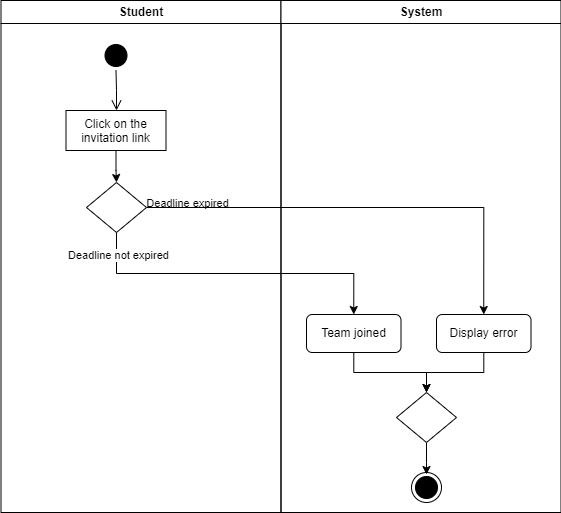
\includegraphics[width=1\linewidth]{Images//Diagrams/StudentReceivesInvitation.png}
    \caption{Diagram for [UC10]}
    \label{fig:enter-label}
\end{figure}

\clearpage

\begin{table}[htbp]
\begin{tabular}{|l|p{12cm}|}
    \hline
    \multicolumn{2}{|l|}{\textbf{[UC11] Educator evaluates a team's project}}\\
    \hline
    Actors & Educator\\
    \hline
    Entry condition & Educator, who has permission to create battles, is already logged in and has navigated to the "Tournament dashboard" page. Educator must have created the battle that he/she is evaluating for.\\
    \hline
    Event flow & The educator clicks on the "Evaluate" button from the "Battle List". From the "Evaluation" pop-up page, the educator selects the team that he/she wants to evaluate from a scroll-down menu. The educator is presented with some useful information that tell him/her how the team achieved a certain score. If the educator is satisfied with the score given automatically by CKB, he/she clicks on "Confirm Score" button. Otherwise, the educator can check the GitHub repository by clicking the "Go to GitHub Repository" button and, eventually, by clicking "Modify Score", he/she can modify the team's score.\\
    \hline
    Exit condition & Educator confirms or modifies and confirms the team's score.\\
    \hline
    Output & \begin{itemize}
        \item Student's personal score is updated
        \item Team's final score is updated
    \end{itemize}\\
    \hline
    Exception & If the score assigned by the educator is $< 0$ or $> 100$, the platform prompts an error to the educator and asks him/her to insert a valid score.\\
    \lasthline
\end{tabular}
\end{table}

\clearpage

\begin{figure}[htbp]
    \centering
    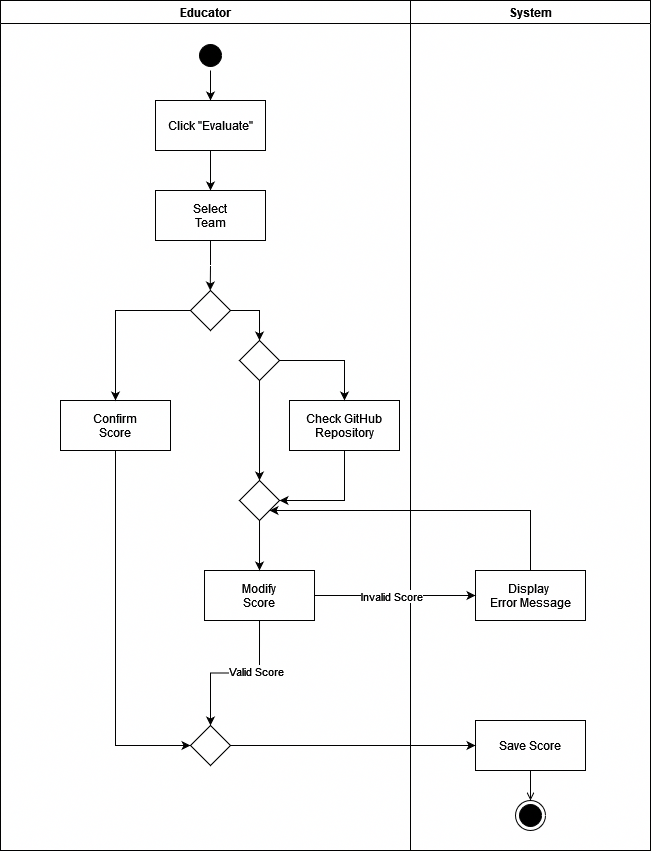
\includegraphics[width=1\linewidth]{Images/Diagrams/Evaluate.png}
    \caption{Diagram for [UC11]}
    \label{fig:enter-label}
\end{figure}

\clearpage

\begin{table}[htbp]
\begin{tabular}{|l|p{12cm}|}
    \hline
    \multicolumn{2}{|l|}{\textbf{[UC12] User checks a student profile}}\\
    \hline
    Actors & User\\
    \hline
    Entry condition & The user is logged in to the system.\\
    \hline
    Event flow & The student clicks on the sidebar, on the icon of the users, this can be done in every moment since the side bar is always present. Once the student is in the page, the platform displays a search bar where he/she can search the student's username he/she wants to check out. A list of possible usernames is then displayed to the user. By clicking the "Show Profile" icon on the right, the platform redirects the user to the student's public profile page.\\
    \hline
    Exit condition & User lands correctly on a student profile page.\\
    \hline
    Output & \begin{itemize}
        \item User can search every student
        \item User can view the public information of a student
    \end{itemize}\\
    \hline
    Exception & If the username inserted by the User does not exist, or if it belongs to an Educator, the platform displays an error message and asks the User to insert a valid username.\\
    \lasthline
\end{tabular}
\end{table}

\clearpage

\begin{figure}[htbp]
    \centering
    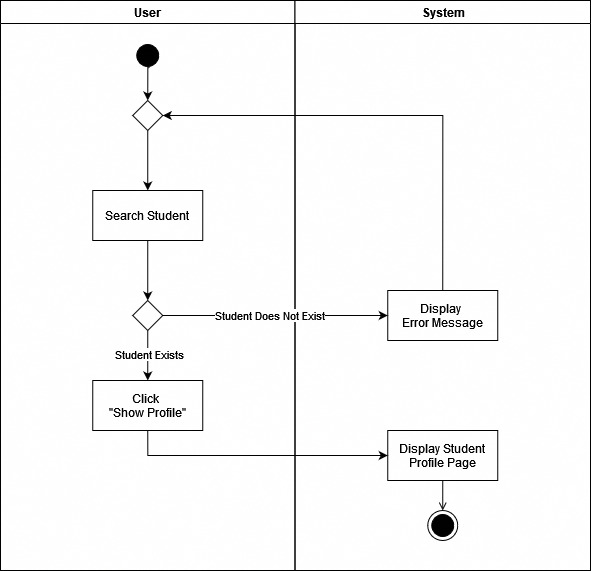
\includegraphics[width=1\linewidth]{Images/Diagrams/CheckProfile.png}
    \caption{Diagram for [UC12]}
    \label{fig:enter-label}
\end{figure}

\clearpage

\begin{table}[htbp]
\begin{tabular}{|l|p{12cm}|}
    \hline
    \multicolumn{2}{|l|}{\textbf{[UC13] Student sends a friend request}}\\
    \hline
    Actors & Student\\
    \hline
    Entry condition & The student is logged in to the system.\\
    \hline
    Event flow & The student clicks on the sidebar, on the icon of the users, this can be done in every moment since the side bar is always present. Once the student is in the page, the platform displays a search bar where he/she can search the friend(s) he/she wants to add. A list of possible usernames is then displayed to the student. By clicking the "Add Friend" icon on the right, the platform sends the request.\\
    \hline
    Exit condition & One or multiple friend requests have been sent successfully.\\
    \hline
    Output & \begin{itemize}
        \item Students can search every student
        \item One or more friend requests are send to to the students
    \end{itemize}\\
    \hline
    Exception & If the username input by the student doesn't exists, the platform prompts an error to the student and asks him/her to insert a valid username.\\
    \lasthline
\end{tabular}
\end{table}

\clearpage

\begin{figure}[htbp]
    \centering
    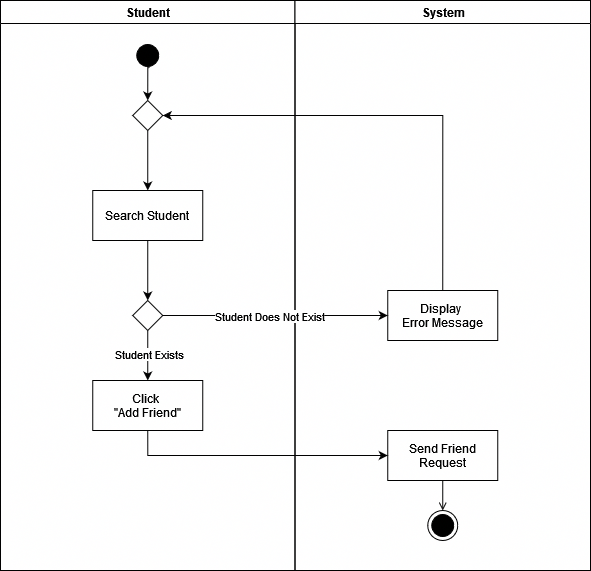
\includegraphics[width=1\linewidth]{Images/Diagrams/FriendRequest.png}
    \caption{Diagram for [UC13]}
    \label{fig:enter-label}
\end{figure}

\clearpage

\begin{table}[htbp]
\begin{tabular}{|l|p{12cm}|}
    \hline
    \multicolumn{2}{|l|}{\textbf{[UC14] Educator closes a tournament}}\\
    \hline
    Actors & Educator\\
    \hline
    Entry condition & Student, who is already logged in, has navigated to the "Educator dashboard" page.\\
    \hline
    Event flow & The educator clicks on the "Close" button, placed in the "Tournament List".\\
    \hline
    Exit condition & Tournament is successfully closed\\
    \hline
    Output & \begin{itemize}
        \item Tournament is closed
        \item Badges are assigned to students
        \item Final scores and rankings are updated
    \end{itemize}\\
    \hline
    Exception & If there are on-going battles in the tournament, the platform prompts an error to the educator and asks him/her to wait for those battles to end.\\
    \lasthline
\end{tabular}
\end{table}

\clearpage

\begin{figure}[htbp]
    \centering
    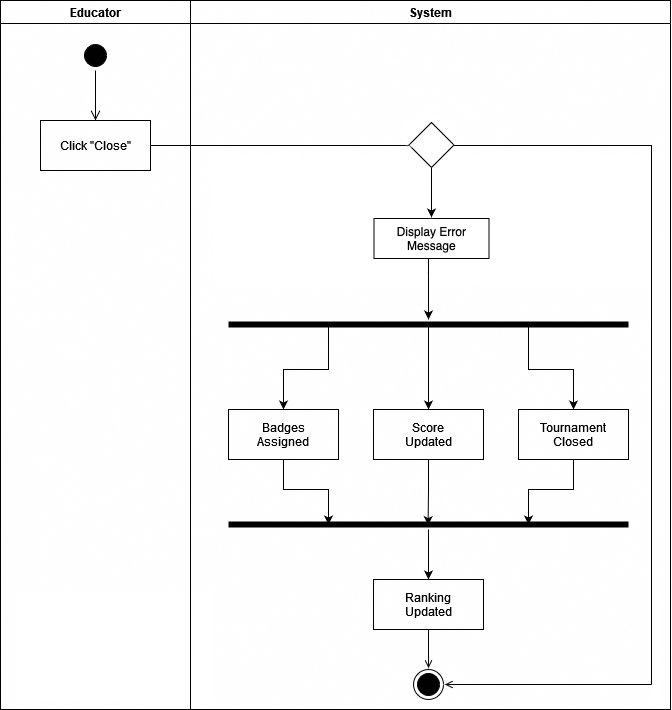
\includegraphics[width=1\linewidth]{Images/Diagrams/CloseTournament.png}
    \caption{Diagram for [UC14]}
    \label{fig:enter-label}
\end{figure}

\clearpage


\begin{table}[H]
\centering
    \begin{tabular}{|c|c|}
    \hline
    \textbf{Requirement} & \textbf{Use Case} \\
    \hline
    \textbf{R1} & UC6\\
    \hline
    \textbf{R2} & UC8\\
    \hline
    \textbf{R3} & UC6\\
    \hline
    \textbf{R4} & UC9, UC12, UC13\\
    \hline
    \textbf{R5} & UC9\\
    \hline
    \textbf{R6} & UC8, UC9\\
    \hline
    \textbf{R7} & UC3\\
    \hline
    \textbf{R8} & UC3\\
    \hline
    \textbf{R9} & UC3, UC5\\
    \hline
    \textbf{R10} & UC3, UC4\\
    \hline
    \textbf{R11} & UC7\\
    \hline
    \textbf{R12} & UC11\\
    \hline
    \textbf{R13} & UC12, UC13\\
    \lasthline
    \end{tabular}
    \caption{Traceability Matrix}
\end{table}

\subsubsection{Requirements}
This subsection provides a concise overview of the goals outlined in Section 1.1, delineating the specific requirements and domain assumptions associated with each goal.
$\\$
\begin{itemize}
    \item \textbf{[G1]: Allow students to subscribe to a tournament}
    \begin{itemize}
        \item \textbf{R1:} The system allows a registered student to accept a tournament invitation.
        \item \textbf{D1:} Users must have a device able to connect to the internet. 
        \item \textbf{D2:} Users give consent to the platform to receive notifications. 
    \end{itemize}
    \item \textbf{[G2]: Allow students to join a battle}
    \begin{itemize}
        \item \textbf{R2:} The system allows a registered student to select a battle to join.
        \item \textbf{R3:} The system allows a registered student retrieve a battles' list for each tournament.
        \item \textbf{D1:} Users must have a device able to connect to the internet.
        \item \textbf{D2:} Users give consent to the platform to receive notifications. 
        \item \textbf{D3:} Students must have GitHub accounts.
    \end{itemize}
    \item \textbf{[G3]: Allow students to form teams}
    \begin{itemize}
        \item \textbf{R4:} The system allows a registered user to retrieve a list of students.
        \item \textbf{R5:} The system allows a registered student to invite a student in his/her team.
        \item \textbf{R6:} The system allows a registered student to create a team.
        \item \textbf{D1:} Users must have a device able to connect to the internet.
        \item \textbf{D2:} Users give consent to the platform to receive notifications. 
    \end{itemize}$\\$
    \item \textbf{[G4]: Allow an educator to create a tournament}
    \begin{itemize}
        \item \textbf{R7:} The system generates a tournament invitation link for all students. 
        \item \textbf{R8:} The system allows a registered educator to set up the tournament parameters.
        \item \textbf{R9:} The system allows a registered educator to grant access to other educators.
        \item \textbf{R10:} The system allows a registered educator to create badges
        \item \textbf{D1:} Users must have a device able to connect to the internet.
    \end{itemize}
    \item \textbf{[G5]: Allow an educator to create a battle}
    \begin{itemize}
        \item \textbf{R11:} The system allows a registered educator to set up the battle parameters.
        \item \textbf{D1:} Users must have a device able to connect to the internet.
    \end{itemize}
    \item \textbf{[G6]: Allow educators to modify a team's score}
    \begin{itemize}
        \item \textbf{R12:} The system displays the automated evaluation score, calculated for the team's project.
        \item \textbf{D1:} Users must have a device able to connect to the internet.
    \end{itemize}
    \item \textbf{[G7]: Allow users to check rankings and scores}
    \begin{itemize}
        \item \textbf{R4:} The system allows a registered user to retrieve a list of students.
        \item \textbf{R13:} The system allows a registered user to see a student's public profile.
        \item \textbf{D1:} Users must have a device able to connect to the internet.
    \end{itemize}
\end{itemize}




\subsection{Performance Requirements}
The system is expected to exhibit a swift response time to prevent any delays that might cause students to miss their deadlines. It is projected that the system will shoulder a manageable workload, as code composition will not occur directly within the platform. Additionally, seamless interaction with the GitHub API is vital to ensure an optimal workflow.

\subsection{Design Constraints}
\subsubsection{Standards Compliance}
The system ensures the web platform's compliance with essential open web standards, including HTML, CSS, and JavaScript, in order to guarantee cross-browser compatibility and accessibility. It also mandates adherence to data protection and privacy regulations like GDPR (General Data Protection Regulation) and CCPA (California Consumer Privacy Act) for the handling of user data. Additionally, the platform is designed to meet accessibility standards, such as WCAG (Web Content Accessibility Guidelines), ensuring its usability for individuals with disabilities. Moreover, it's imperative that the web platform functions flawlessly and maintains visual consistency across a variety of web browsers, such as Chrome, Firefox, Safari, and Edge.
\subsubsection{Hardware Limitation}
In terms of hardware necessities, a computer with an internet connection is sufficient.
\subsubsection{Any other constraints}
The sole additional necessity, which only applies to the students, for platform usage is the possession of a GitHub account.
\subsection{Software System Attributes}
\subsubsection{Reliability}
The system must minimize downtime to allow users the flexibility to learn coding at their convenience and meet their deadlines without disruption.
\subsubsection{Availability}
The system's availability should be maximized, aiming for a minimum uptime of 97\%.
\subsubsection{Security}
Communication between parties is secured through encryption and utilizes a secure channel via the SSL protocol. Additionaly it assures compliance with security standards like OWASP (Open Web Application Security Project) guidelines to protect against common web application vulnerabilities, including cross-site scripting (XSS), SQL injection, and cross-site request forgery (CSRF). Interaction with the GitHub API is also fortified to ensure fault tolerance. Additionally, the database is designed to ensure that all operations are authorized, preventing unauthorized modifications, such as a student altering a grade assigned by an educator.
\subsubsection{Maintainability}
The system is designed to facilitate the effortless integration of future functionalities with minimal effort. The chosen design techniques must prioritize and ensure a high level of re-usability.

\subsubsection{Portability}
The system is engineered to support smooth portability in case of changes to the hosting databases or individual hardware components.

\clearpage

\section{Formal analysis using Alloy}

\begin{lstlisting}
    open util/integer

    abstract sig User {
        username: one String,
        password: one String,
        email: one String,
        institutionalID: one Int
    }

    sig DateTime {
        day: one Int,
        month: one Int,
        year: one Int
    }

    sig TournamentRegistration{
        tournament: one Tournament,
        date: one DateTime
    }

    sig BattleRegistration{
        battle: one Battle,
        date: one DateTime
    }
   
    sig Student extends User{
        gitHub: one String,
        tournaments: set TournamentRegistration,
        battles: set BattleRegistration
    }

    sig Educator extends User{}

    sig Team{
        name: one String,
        members: some Student,
        repository: one String,
        lastSub: one LastSubmission
    }

    sig LastSubmission{
        name: one String,
        code: one File,
        date: one DateTime
    }

    sig File {}
    
    sig Tournament{
        creator: one Educator,
        collaborators: set Educator,
        title: one String,
        regDeadline: one DateTime,
        language: one String,
        badges: set Badge,
        battles: set Battle,
      
    }{
        //The tournament creator cannot be a collaborator
        not creator in collaborators 
    }
   
    sig Badge{
        name: one String,
        rules: some Rule,
	tournament: one Tournament
    }
    
    sig Rule{
        variables: some Int,
	badge: one Badge
    }

    sig Battle{
        name: one String,
        minNumber: one Int,
        maxNumber: one Int,
        regDeadline: one DateTime,
        subDeadline: one DateTime,
        enrolledTeams: set Team,
        creator: one Educator,
	tournament: one Tournament
    }{
        //The minimum number for the team members must be smaller or equal than the maximum number
        minNumber <= maxNumber

        //The registration deadline must be before the submission deadline
        regDeadline.day < subDeadline.day 

        //The same team cannot participate at the same battle more than once
        no disj t1, t2 : enrolledTeams |  t1.name =  t2.name
    }

    //FACTS

    // Each user has a unique username
    fact{
        all u1, u2: User | u1 != u2 implies u1.username != u2.username
    }

    // Each user has a unique email address
    fact{
        all u1, u2: User | u1 != u2 implies u1.email != u2.email
    }

    // Each user has a unique institutional ID
    fact{
        all u1, u2: User | u1 != u2 implies u1.institutionalID != u2.institutionalID
    }
   
    //Every student must register to a battle before the registration deadline
    fact{
        all r : BattleRegistration | r.date.day < r.battle.regDeadline.day
    }

    // Every student must have a unique GitHub account
    fact{
        no disj s1, s2 : Student | s1.gitHub = s2.gitHub
    }

    //Each team has a unique GitHub repository
    fact{
        no disj t1, t2 : Team | t1.repository = t2.repository
    }
  
    //A student cannot participate in the same team more than once
    fact{
        all t : Team | no disj m1, m2 : t.members | m1.institutionalID = m2.institutionalID
    }

    // A student cannot register himself in the same tournament more than once
    fact{
        all s : Student | no disj t1, t2 : s.tournaments | t1.tournament = t2.tournament
    }

    //Every student must register to a tournament before the registration deadline
    fact{
        all s : Student | all r : s.tournaments | r.date.day < r.tournament.regDeadline.day
    }

    //Each battle belongs to a single tournament
    fact {
        all disj t1, t2 : Tournament | no b1 : Battle | b1 in t1.battles and b1 in t2.battles
    }
    
    //Every battle in a tournament has a reference to that tournament
    fact{
	all t : Tournament | all b : Battle | b.tournament = t iff b in t.battles
    }

    //Every badge in a tournament has a reference to that tournament
    fact{
	all t : Tournament | all b : Badge | b.tournament = t iff b in t.badges
    }

    //Every rule can only be associated with one badge
    fact{
	all r : Rule | all b : Badge | r.badge = b iff r in b.rules
    }

    //Each student can participate to a battle with a single team
    fact {
        all s : Student, b : Battle | no disj t1, t2 : b.enrolledTeams | s in t1.members and s in t2.members
    }

    //Every team's last submission must be before the submission deadline
    fact {
        all b : Battle, t : Team | t.lastSub.date.day < b.subDeadline.day
    }

    //Each tournament has a unique title
    fact{
        no disj t1, t2 : Tournament | t1.title = t2.title
    }
    
    //Each battle in a tournament has a unique name
    fact{
        all t : Tournament | no disj b1, b2 : t.battles | b1.name = b2.name
    }

    //Each badge in a tournament has a unique name
    fact{
        all t : Tournament | no disj b1, b2 : t.badges | b1.name = b2.name
    }


pred show{
	#Student > 1
	#Tournament > 1
	#Battle>1
	#Educator>1
	#Badge > 1
	#Team > 1
}
run show for 10 but exactly 10 String
\end{lstlisting}

\clearpage

\begin{figure}
    \centering
    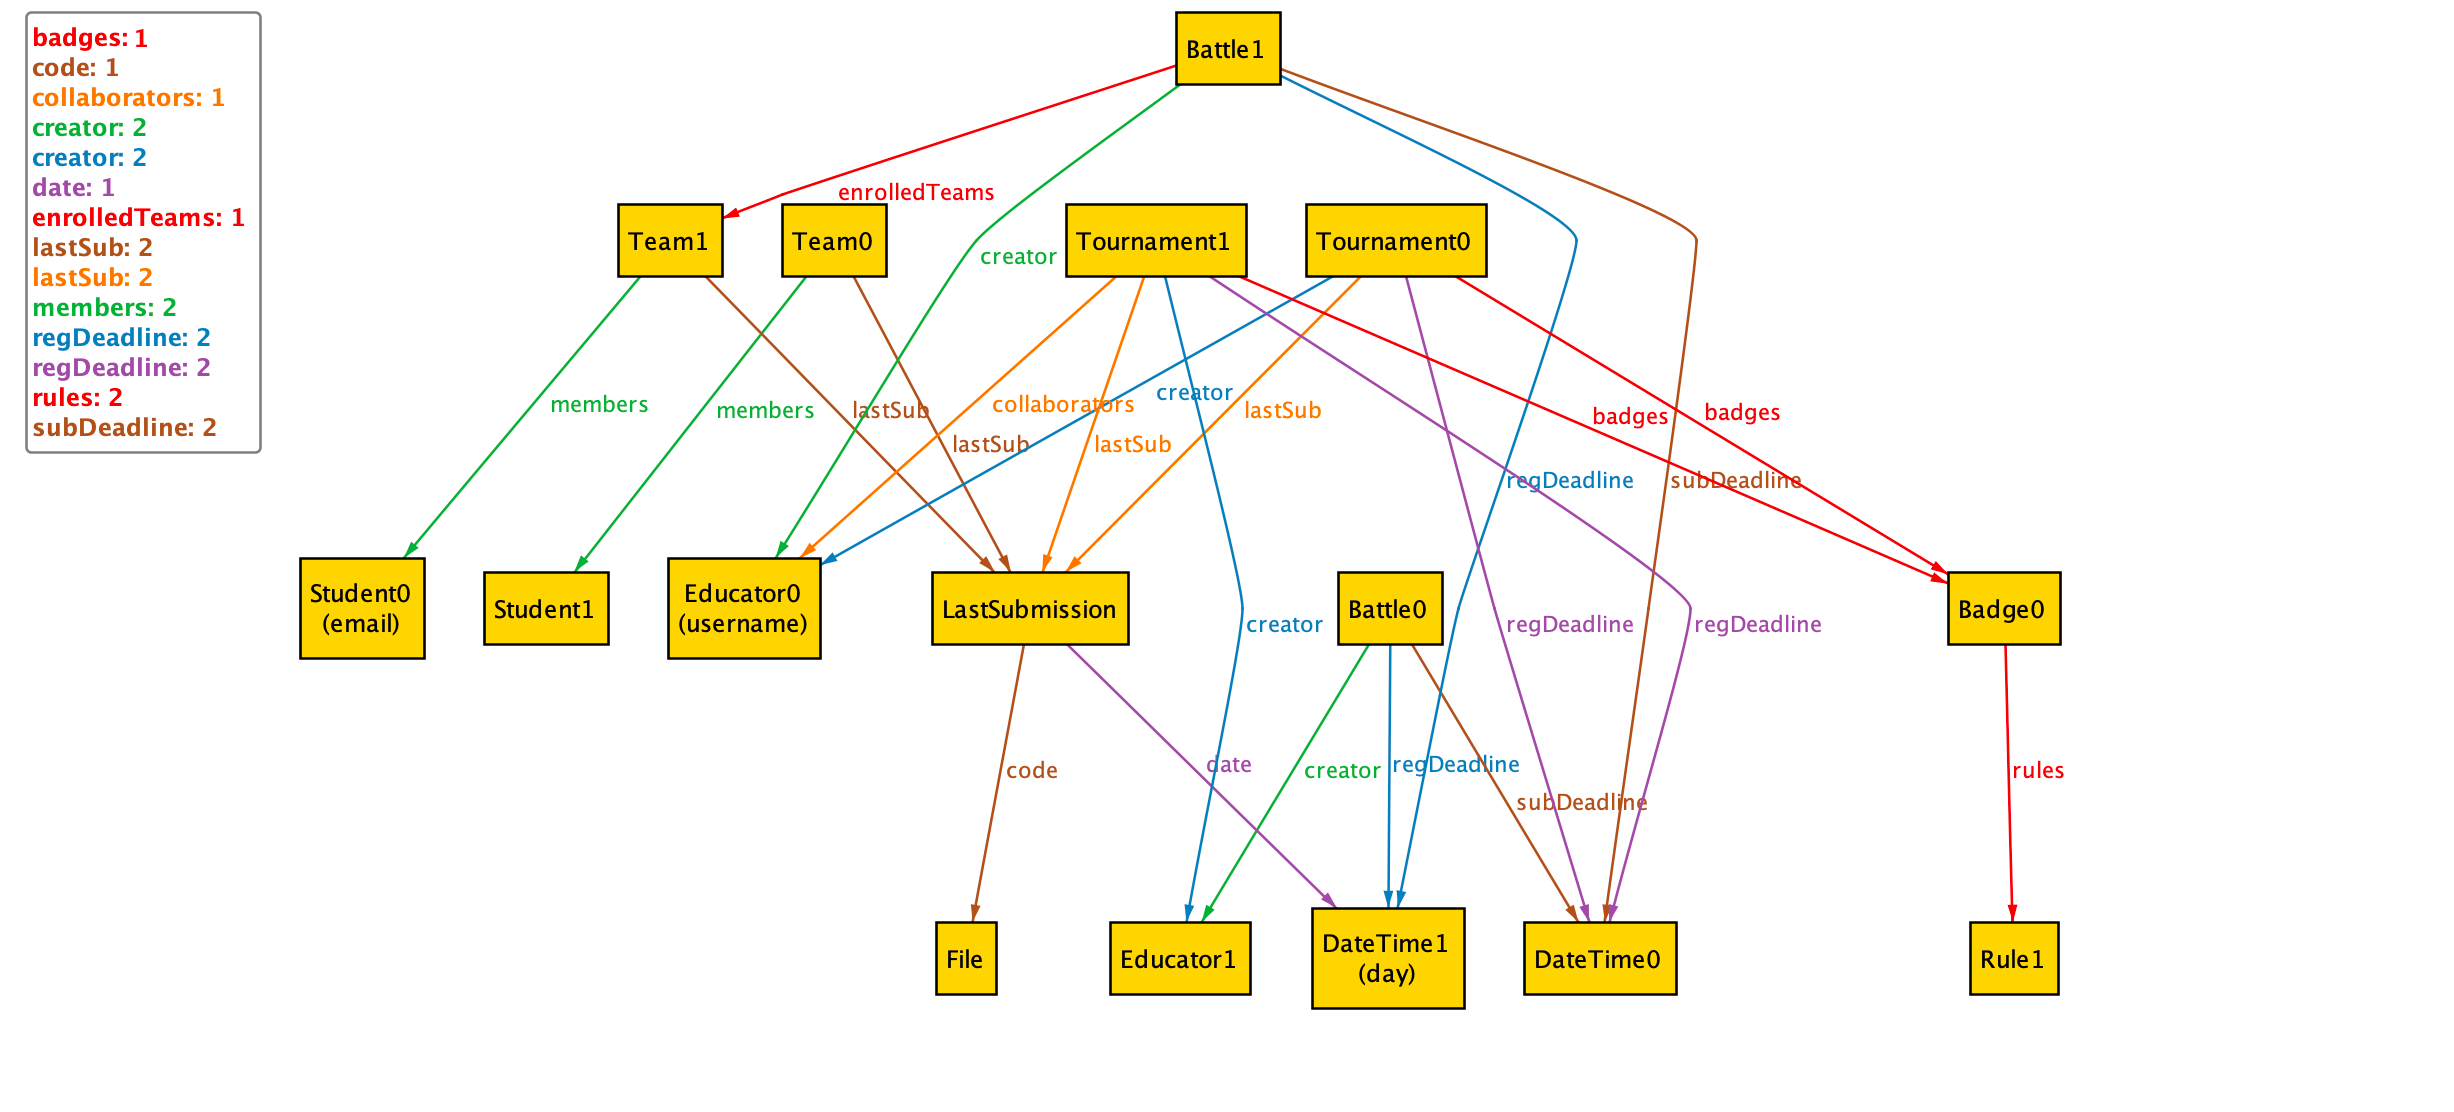
\includegraphics[width=1\linewidth]{Images//Diagrams/Alloy.png}
    \caption{Alloy Diagram}
    \label{fig:enter-label}
\end{figure}

\clearpage

\section{Effort spent}
\begin{table}[H]
\centering
\begin{tabular}{|c|c|c|c|c|}
\hline
\textbf{Student} & \textbf{Section 1} & \textbf{Section 2} & \textbf{Section 3} & \textbf{Section 4} \\
\hline
Filippo Gentili & 3h & 7h & 15h & 7h \\
\hline
Emanuele Greco & 3h & 8h & 14h & 7h\\
\hline
Marco Giulio Grilli & 3h & 9h & 13h & 7h \\
\hline
\end{tabular}
\end{table}
\section{References}
In the RASD-Document we have used the following references:

$\\$Websites that have a similar use case:
\begin{itemize}
    \item \href{https://www.leetcode.com}{LeetCode}
    \item \href{https://www.hackerrank.com}{HackerRank}
    \item \href{https://www.codewars.com}{CodeWars}
    \item \href{https://www.github.com}{GitHub}
\end{itemize}

$\\$Websites used for the mock ups:
\begin{itemize}
    \item \href{https://www.moqups.com}{Moqups}
    \item \href{https://www.designs.ai}{Designs}
    \item \href{https://www.looka.com}{Looka}
\end{itemize}

$\\$Websites used for the diagrams:
\begin{itemize}
    \item \href{https://www.draw.io}{Draw}
\end{itemize}

\end{document}